\documentclass[10pt]{scrartcl}
\usepackage[slantfont,boldfont]{xeCJK}
\usepackage{xltxtra,fontspec,xunicode}
% 设置中文字体
\setCJKmainfont[BoldFont=SimHei,ItalicFont=KaiTi]{SimSun}   % 设置缺省中文字体
\setCJKmonofont[BoldFont=SimHei]{SimSun}   % 设置中文等宽字体
\setCJKsansfont{KaiTi}
\usepackage[]{xkeyval,polyglossia}
\usepackage[a5paper,top=2cm, bottom=2cm, left = 2.5cm, right=2cm]{geometry}
\usepackage[]{csquotes}
\usepackage[]{titlesec}
\usepackage[]{url}
\usepackage[]{paralist}
\usepackage[absolute]{textpos}
\usepackage[]{rotating}
\usepackage{amsmath}
\usepackage{listings}
\lstset{%language=C,
%        tabsize=2,
%        keywordstyle=\color{blue},
%        numbers=left,
%        stepnumber=1,
%       numberstyle=\tiny,
%        keepspaces=false,
%        breakindent=2pt,
%       basicstyle=\footnotesize,
%        showspaces=false,
%        flexiblecolumns=true,
        breaklines=true,
%        breakautoindent=true,
%        breakindent=1em,
%        escapeinside={/*@}{@*/},
%        frameround=tttt,
%        frame=trBL,
%       escapeinside=``,
}

\usepackage{subfigure}
\usepackage{float} 

%设置脚注
\renewcommand{\thefootnote}{\arabic{footnote}}
\setcounter{footnote}{0}

 
\usepackage[]{scrpage2}
\usepackage[]{blindtext}
 
\pagestyle{scrheadings}
\setheadsepline[\textwidth]{0.25pt}{}
 
\ohead{\headmark}
\ofoot[\pagemark]{\pagemark}
\cfoot{}
\chead{}
\ihead{14307130092 李英伟}
 
\usepackage{xcolor}
\definecolor{msdarkblue}{RGB}{54,95,145}
\definecolor{msblue}{RGB}{79,129,189}
 
%\titleformat{\section}[form]{layout}{labellayout}{abstand}{davorcode}[danachcode]
\titleformat{\section}[hang]{\color{msdarkblue}\Large\sffamily\bfseries}{}{0pt}{\vspace*{-6pt}}
\titleformat{\subsection}[hang]{\color{msblue}\large\sffamily\bfseries}{}{0pt}{\vspace*{-4pt}}
\titleformat{\subsubsection}[hang]{\color{msblue}\normalsize\sffamily\bfseries}{}{0pt}{}
 
\setsansfont[ItalicFont={Cambria Italic},BoldFont={Cambria Bold},BoldItalicFont={Cambria Bold Italic}]{Cambria}
\setmainfont[ItalicFont={Calibri Italic},BoldFont={Calibri Bold},BoldItalicFont={Calibri Bold Italic}]{Calibri}
\setmonofont[ItalicFont={Consolas Italic},BoldFont={Consolas Bold},BoldItalicFont={Consolas Bold Italic}]{Consolas}
 
\usepackage{indentfirst}
\setmainlanguage{english}
\setlength{\parindent}{2em}
\setlength{\parskip}{1em}
 
\usepackage{unicode-math}
\setmathfont{Cambria Math}

\bibliographystyle{plain}

\begin{document}
 
\setlength{\TPHorizModule}{1.2mm}
\setlength{\TPVertModule}{1mm}
 
\begin{titlepage}
~
\begin{textblock}{50}(-10,-10)
  \begin{color}{msdarkblue}
    \rule{3cm}{25cm}    
  \end{color}
\end{textblock}
 
% Logo white
\begin{textblock}{130}(30,30)
 
{\noindent\Huge\bfseries 数据结构大作业 \\ \\ Data Structure Project } \\[0.1em]
 
{\noindent\huge\bfseries  时空数据管理\\[0.05em] Spatio-temporal Data Management }\\[5em]
 
{\noindent\Large\bfseries 李英伟 \\ 14307130092}\\[1em]

{\noindent\Large \today }
 
\end{textblock}
 
 
\begin{textblock}{20}(12,200)
\begin{rotate}{90}
{\huge\bfseries \textcolor{white}{}}
\end{rotate}
\end{textblock}
 
\end{titlepage}
 
 
\tableofcontents
 
\clearpage

\section{[显著]独立性声明}
除了以下提到的以外都是自己独立完成的:
\begin{enumerate}
    \item pugixml是一个解析XML的库,官方网站:pugixml.org
    \item 使用了boost库中的rtree
    \item plot\_config.xml、ShortestPath.conf两个文件分别是用来配置地图配色和车速的,修改自github.com/Orthocenter/YuxinMap
    \item 实验中所使用的红黑树调用了STL中的map
    \item 使用了opencv2库来画点和直线
    \item 在自己实现三维kd树前曾经问过林禹全同学二维kd树的做法,并且看了他二维kd树的实现,所以代码可能会有点相似,但是也是自己独立完成的,毕竟二维kd树复制过来是不能变成三维的。在这里非常感谢林禹全同学的帮助。
\end{enumerate}


\section{地图数据的抓取和处理}
\subsection{地图数据结构的建立和地图的绘制}

\subsubsection{做法概要}
在读取上海地图时使用了pugixml对上海地图文件进行了解析。使用了boost库中的R树和std库中的map对读取出的点和道路的数据进行预处理并且存储。当请求一块范围内的地图时(即给出矩形对角线上两点的经纬度坐标时),通过之前的数据结构得到要画线和多边形的信息,通过opencv2库中的画点和画多边形的函数,最终画出地图。

\subsubsection{亮点}
\begin{enumerate}
\item 通过R树可以快速的查出要画的小区域中的点,并且通过预处理O(1)的找到与相邻的点构成的一小段路的相关信息,即可快速画出对应小区域中的信息,而不用把全图都扫一遍。
\item 地图层次分明。地图是有层次的,如高架路在最上面,下面是普通的路,再下面是地下通道,最后是河流等。为了画出层次正确的地图,把找到的线和多边形按预处理出来的层次进行排序,按层次从低到高依次绘制。为了描出路的边,可以先画一条比路粗两个单位的线,再在上面画路,就可以达到描边的效果,放在有层次的地图中要注意对于相同层次,要统一先画底色,再统一画线,这样可以表现出同一层次道路相互交叉的效果。
\item 配色美观。效果见Figure1。
\end{enumerate}
\begin{figure}[htbp] 
\centering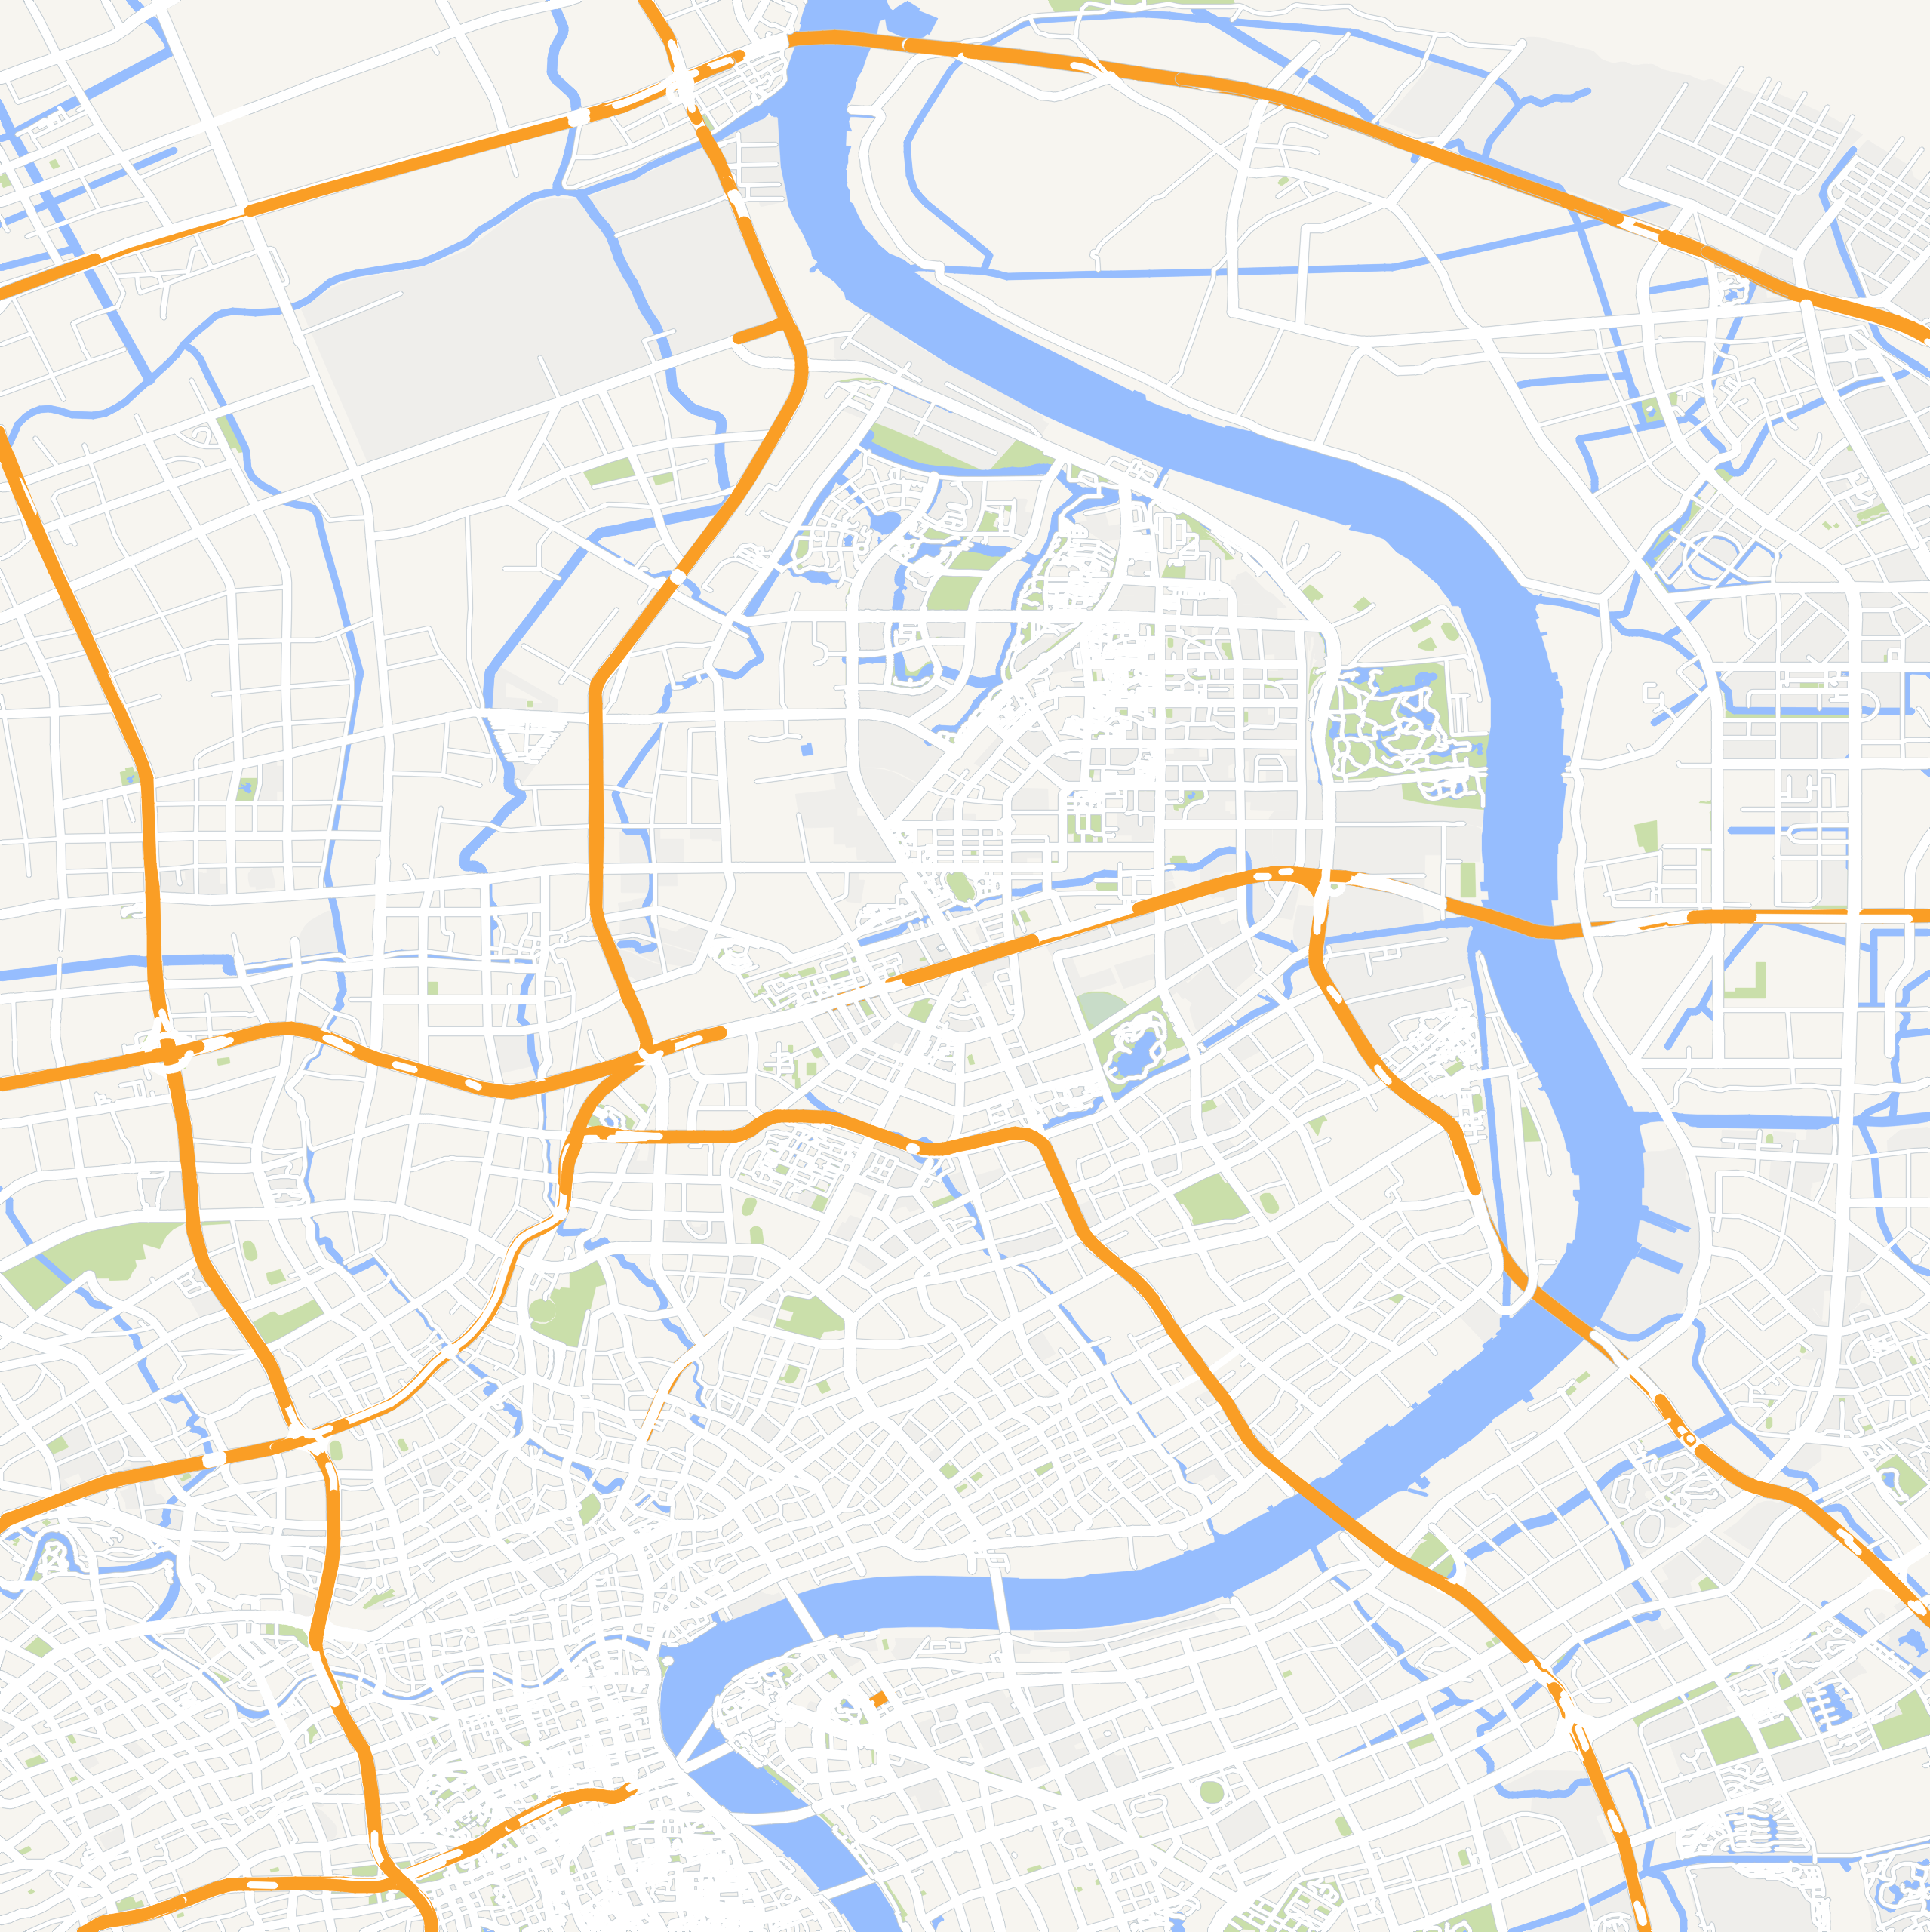
\includegraphics[width=2.9in]{image} 
\caption{地图效果图}\label{fig:1} 
\end{figure} 

\subsubsection{缺点和改进方法}
因为时间有限,不可能做到尽善尽美,所以有些有待解决的次要一些的问题只能提供一个解决方法。
\begin{enumerate}
\item 索引选择的数据结构有待改进:R树虽然很强大,可以支持动态插入点、插入矩形框。在实际应用环境中如果地图是每天动态更新的,那么R树是会有优势的。但是如果对地图的更新度的要求不是很高,我们完全可以采用静态的数据结构,可以达到更快更好的效果,在报告的后半部分详细的讨论了高维空间索引的问题。以后有时间可以考虑换一种更合适的数据结构。
\item 地图的渲染速度较慢,原因有三:一是绘图比较细致,为了描出道路的边几乎花了二倍的时间;二是CPU渲染速度较慢,可以考虑使用GPU绘图;三是当加载全图时把所有细节都画了出来,为了加速可以只画主要的路和建筑物。
\end{enumerate}

\subsection{最短路算法的实验}
\subsubsection{做法概要}

本PJ实现了三种不同的最短路算法(SPFA、dijkstra、A*),得到了两种意义下的最短路:路程最短的路和所花时间最短的路。两者的不同之处在于前者的边权是两点之间的实际距离,而后者的边权是两点之间的实际距离除以依据这条道路等级而假设的速度(即经过这段所需要的时间)。在所花时间意义下得最短路还有躲避拥堵的功能,即如果指定某条路为拥堵路段,那么这条路上行驶的速度就会减小到一个很小的值。有一个想法是把图中入度为2的点去掉,这样道路上的总点数就会从25000个降到8000个,这样虽然可以降低计算最短距离的时间,但是把点画在图上时会比较复杂,而且因为点数过少,所以不能很好的比较各算法之间的时间复杂度。

大致了解了孙老师上课时推荐的SIGMOD2013的最短路算法\cite{DBLP:journals/corr/abs-1304-4661},通过和张睿哲同学的讨论认识到这种算法由于占用空间过大,并不能在普通的笔记本电脑上进行实验。

\subsubsection{性能对比分析}

SPFA、Dijkstra和A*都是最平常的做法,不再赘述,其中A*所使用的估价函数是两点之间直线距离(路程最短路)和两点之间最短距离除以最高车速(时间最短路)。

性能实验方法:随机在路上找起点和终点,然后分别用六种方法(时间意义下和路程意义下得SPFA、Dijkstra和A*)进行最短路的计算,循环一定次数后得到平均运行时间,结果如下:

\begin{tabular}{|l|r|r|r|}
\hline
循环次数    & 100次  & 500次   & 1000次 \\
\hline
[SPFADist] & 4213ms & 3796ms  & 4593ms \\
\hline
[DijkDist] & 72ms   & 66ms    & 85ms \\
\hline
[A*  Dist] & 19ms   & 18ms    & 23ms \\
\hline
[SPFATime] & 1982ms & 2176ms  & 2201ms \\
\hline
[DijkTime] & 59ms   & 65ms    & 71ms \\
\hline
[A*  Time] & 25ms   & 24ms    & 32ms \\
\hline
\end{tabular}

可以看出总体而言SPFA表现最差,A*表现最好。在距离意义下A*是Dijkstra的4倍,而在时间意义下A*是Dijkstra的两倍多,原因是上述估价函数是基于距离进行估价的,所以在时间意义上表现不够好。也曾经尝试过改变A*的估价函数,试图加上速度这一因素,但是效果还没有最初的效果好。

\subsubsection{亮点}
\begin{enumerate}
\item 两种最短路和避免拥堵的情况都考虑到了实际情况的应用,路程最短路可以作为步行的结果,时间最短路可以作为交通工具为汽车时的结果,还考虑了堵车的情况。
\item 考虑了单行道,能否掉头,能否左转等情况,不会出现违反交通规则的路线。
\end{enumerate}

\subsubsection{待改进点}
\begin{enumerate}
\item 最短路算法中堆的实现采用了stl中的priority\_queue,虽然复杂度上没有变化,但是因为没有及时删除堆内无用元素,所以常数比较大,并没有达到最优的性能。以后可以考虑手写堆,或者用斐波那契堆。
\item 没有尝试双向Dijkstra等算法。
\end{enumerate}

\subsubsection{效果展示}
从张江校区往返邯郸校区,考虑当前杨浦大桥是否拥堵的四种结果如下图所示。可以看出步行距离大概是18km,假设全部道路顺畅的话大概需要23分钟,如果杨浦大桥拥堵,那么到张江需要29分钟,从张江出发需要27分钟。而且四幅图走的路线也不完全一样。上面的时间(可能会稍短一些,因为考虑的是道路非常通畅时的情况)和距离和高德地图给出的基本一致。

\begin{figure}[H]
\centering
\subfigure[最短路展示]{
\label{Fig.sub.1}
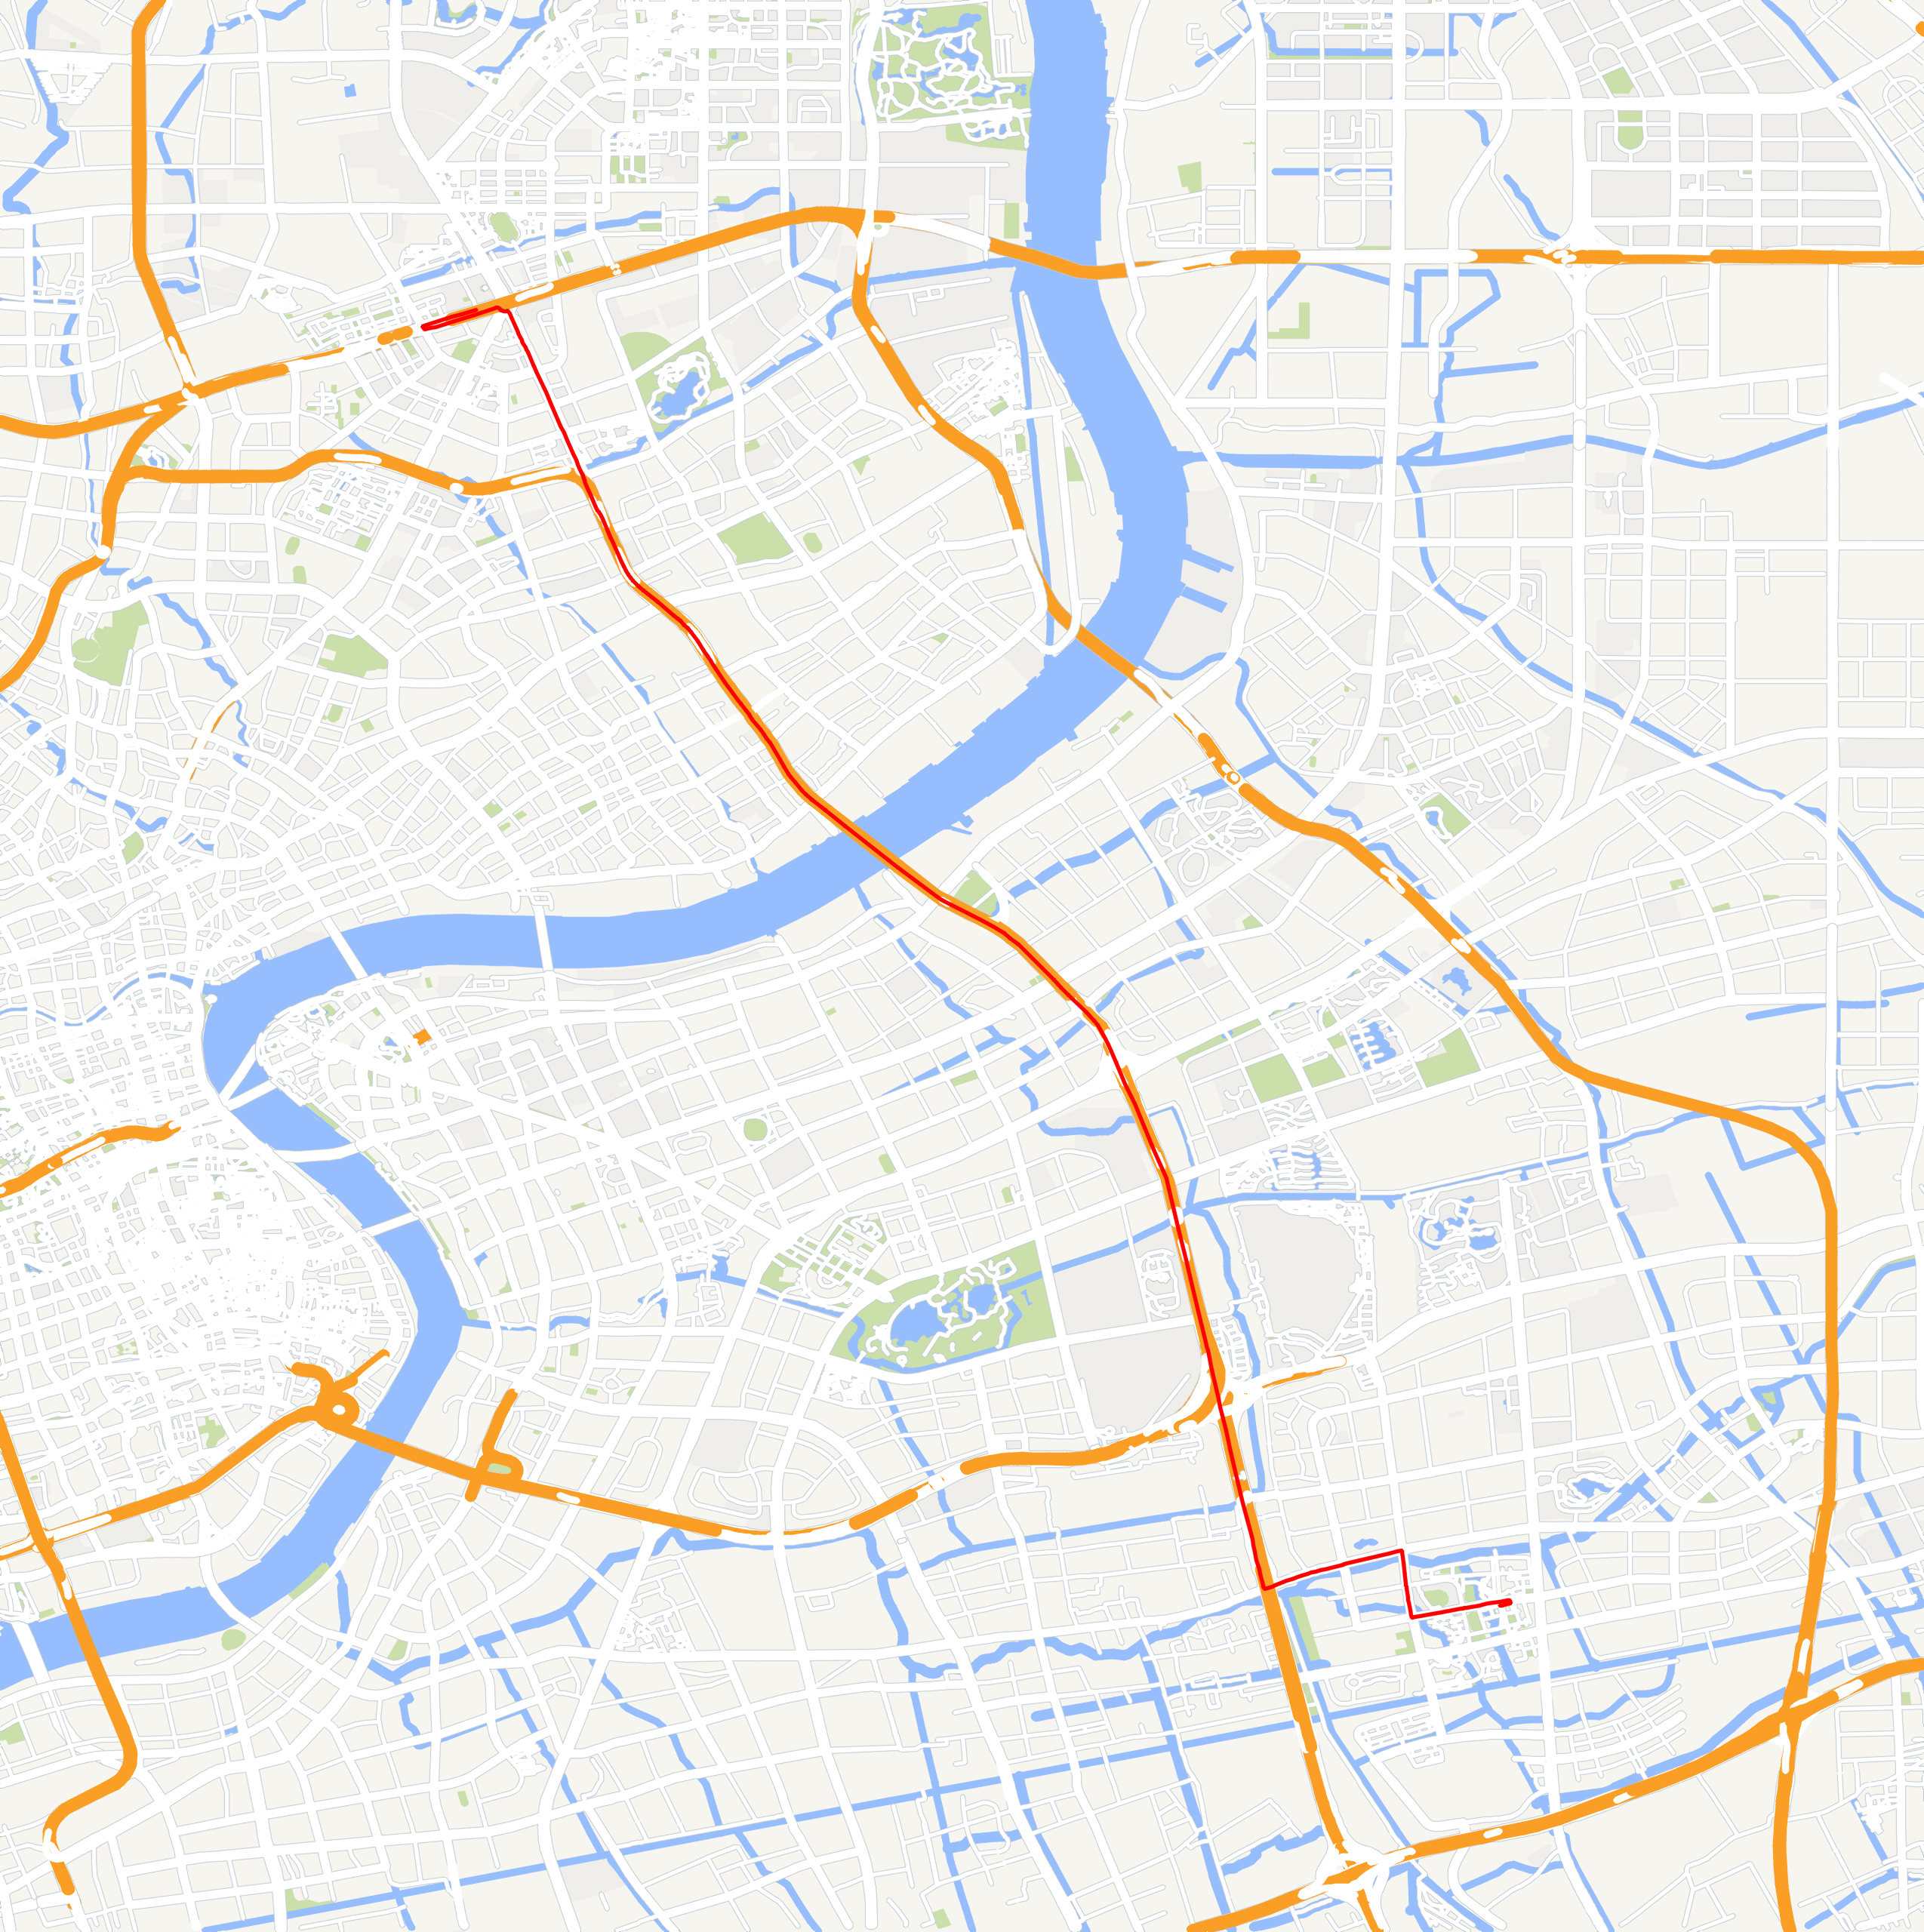
\includegraphics[width=0.4\textwidth]{邯郸到张江不绕}}
\subfigure[相关信息]{
\label{Fig.sub.2}
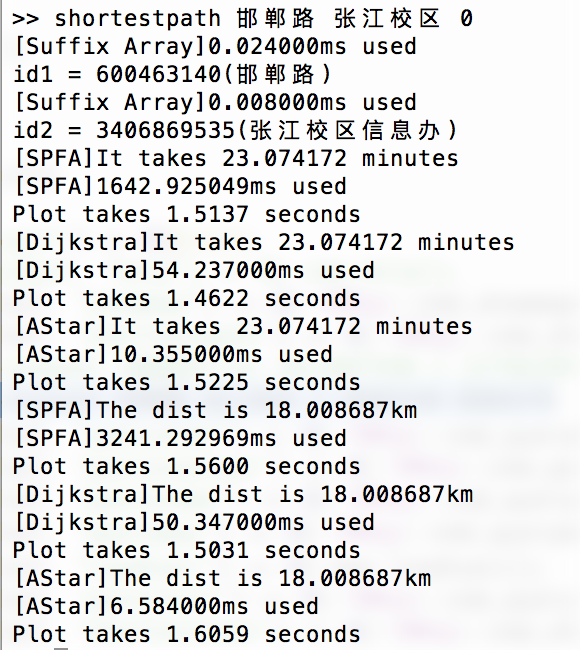
\includegraphics[width=0.4\textwidth]{邯郸到张江不绕路}}
\caption{邯郸到张江最短路}
\label{Fig.lable1}
\end{figure}

\begin{figure}[H]
\centering
\subfigure[最短路展示]{
\label{Fig.sub.3}
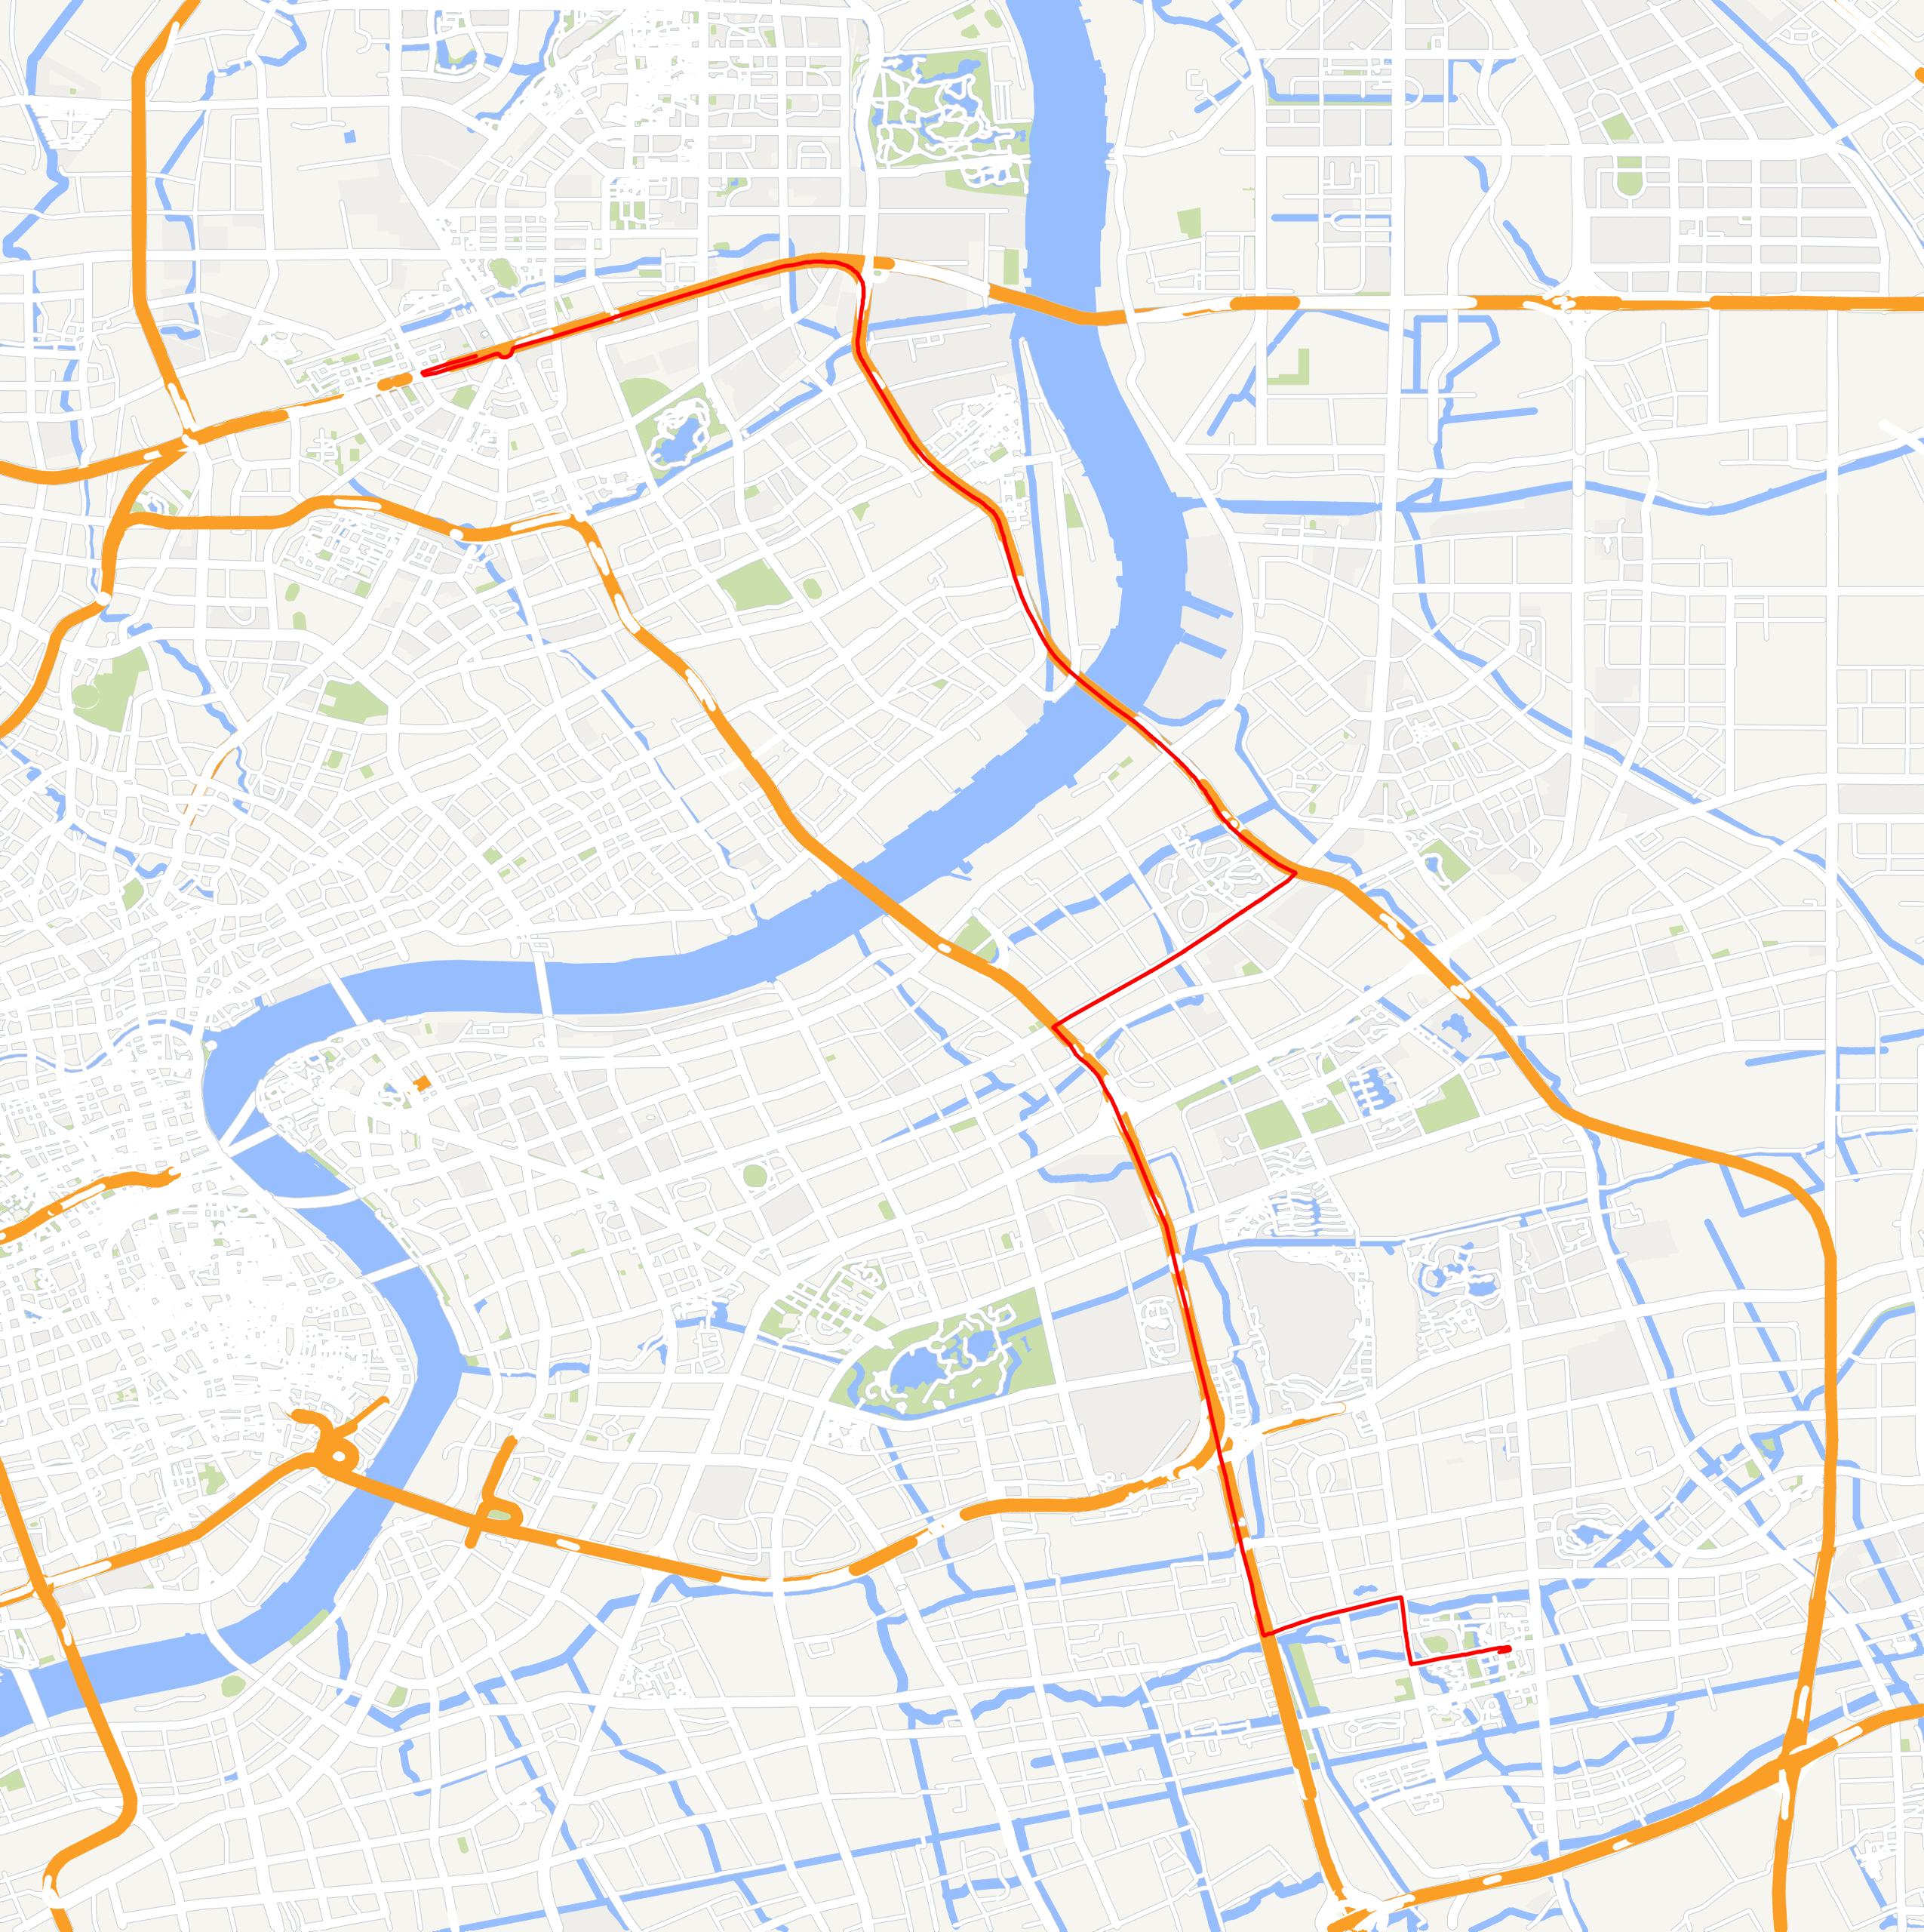
\includegraphics[width=0.4\textwidth]{邯郸到张江绕}}
\subfigure[相关信息]{
\label{Fig.sub.4}
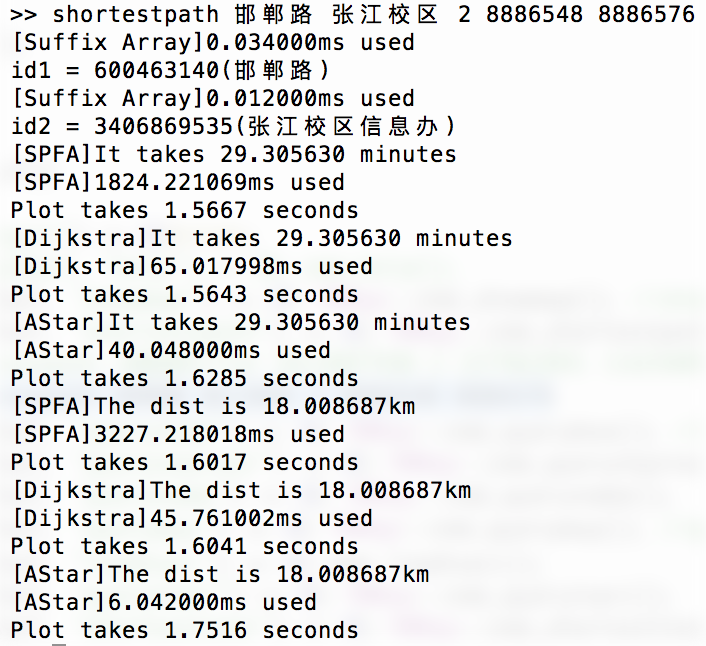
\includegraphics[width=0.4\textwidth]{邯郸到张江绕路}}
\caption{邯郸到张江最短路(躲避拥堵的杨浦大桥)}
\label{Fig.lable2}
\end{figure}

\begin{figure}[H]
\centering
\subfigure[最短路展示]{
\label{Fig.sub.5}
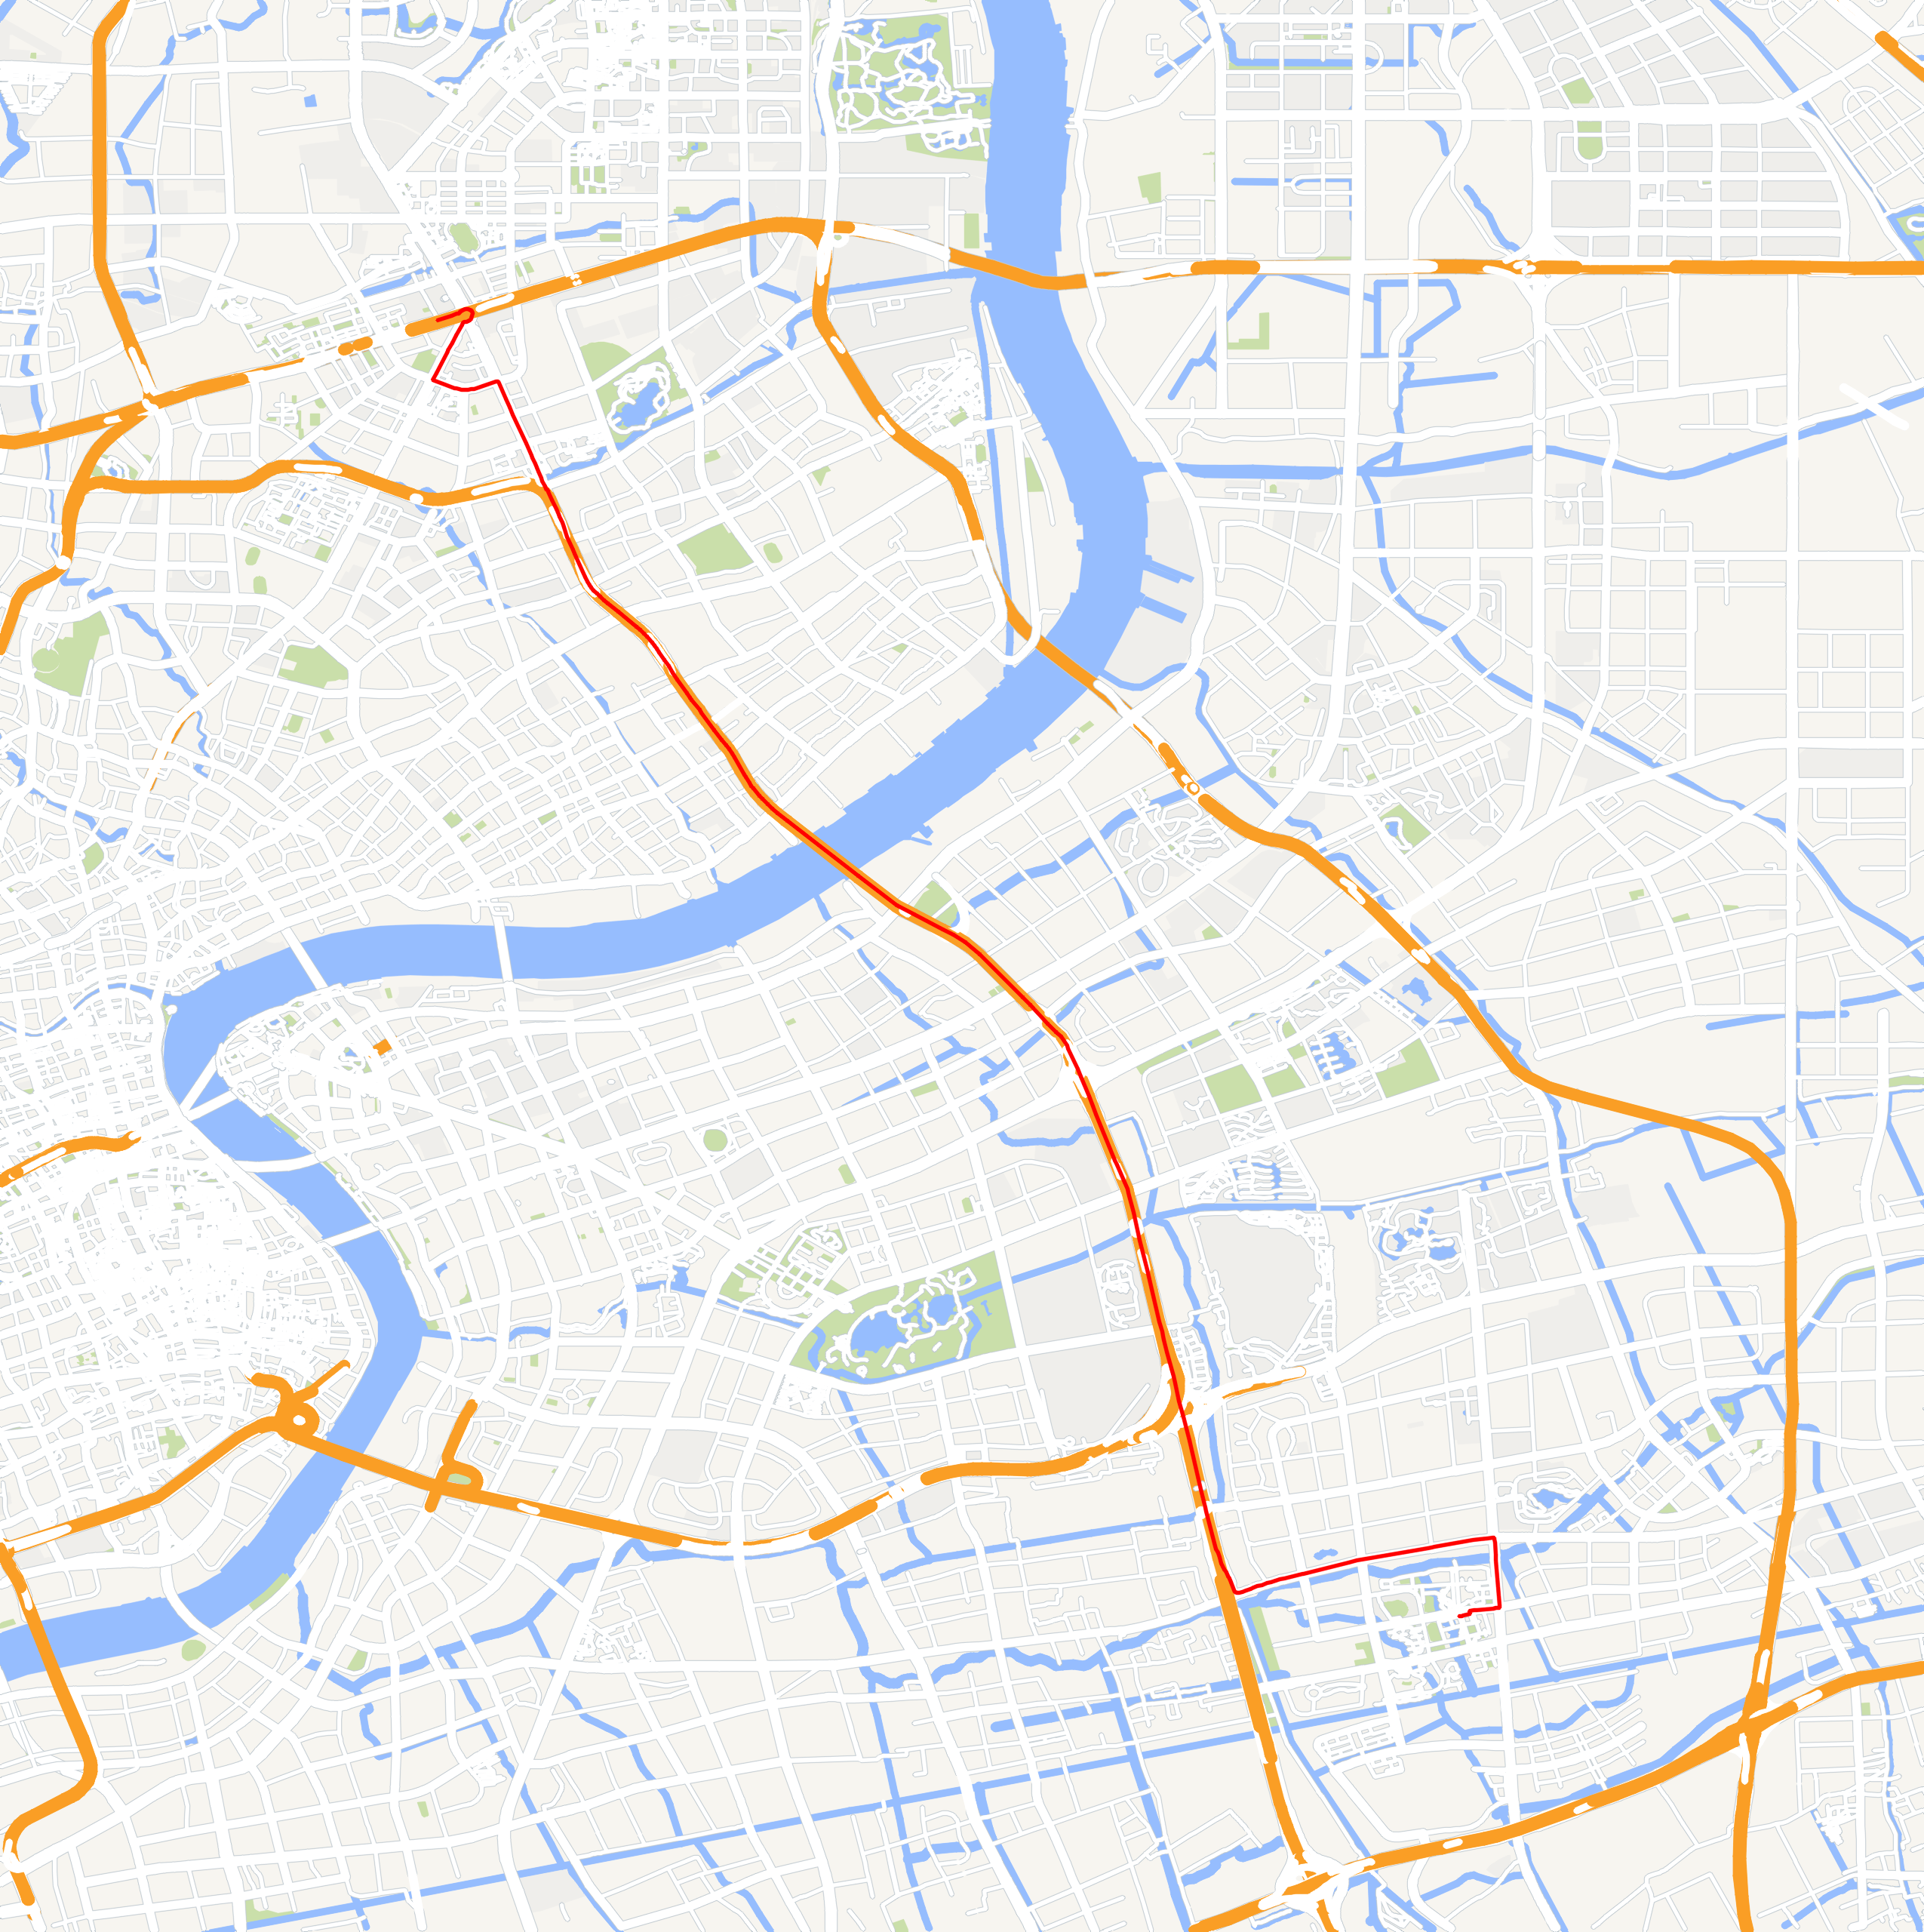
\includegraphics[width=0.4\textwidth]{张江到邯郸不绕}}
\subfigure[相关信息]{
\label{Fig.sub.6}
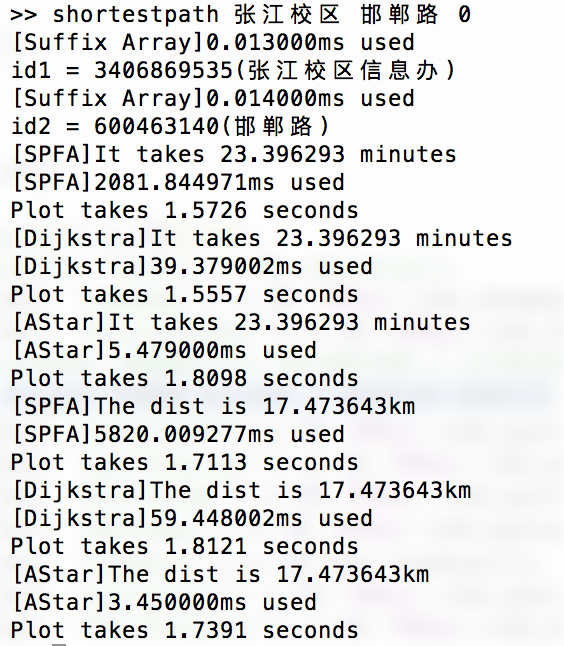
\includegraphics[width=0.4\textwidth]{张江到邯郸不绕路}}
\caption{张江到邯郸最短路}
\label{Fig.lable3}
\end{figure}

\begin{figure}[H]
\centering
\subfigure[最短路展示]{
\label{Fig.sub.7}
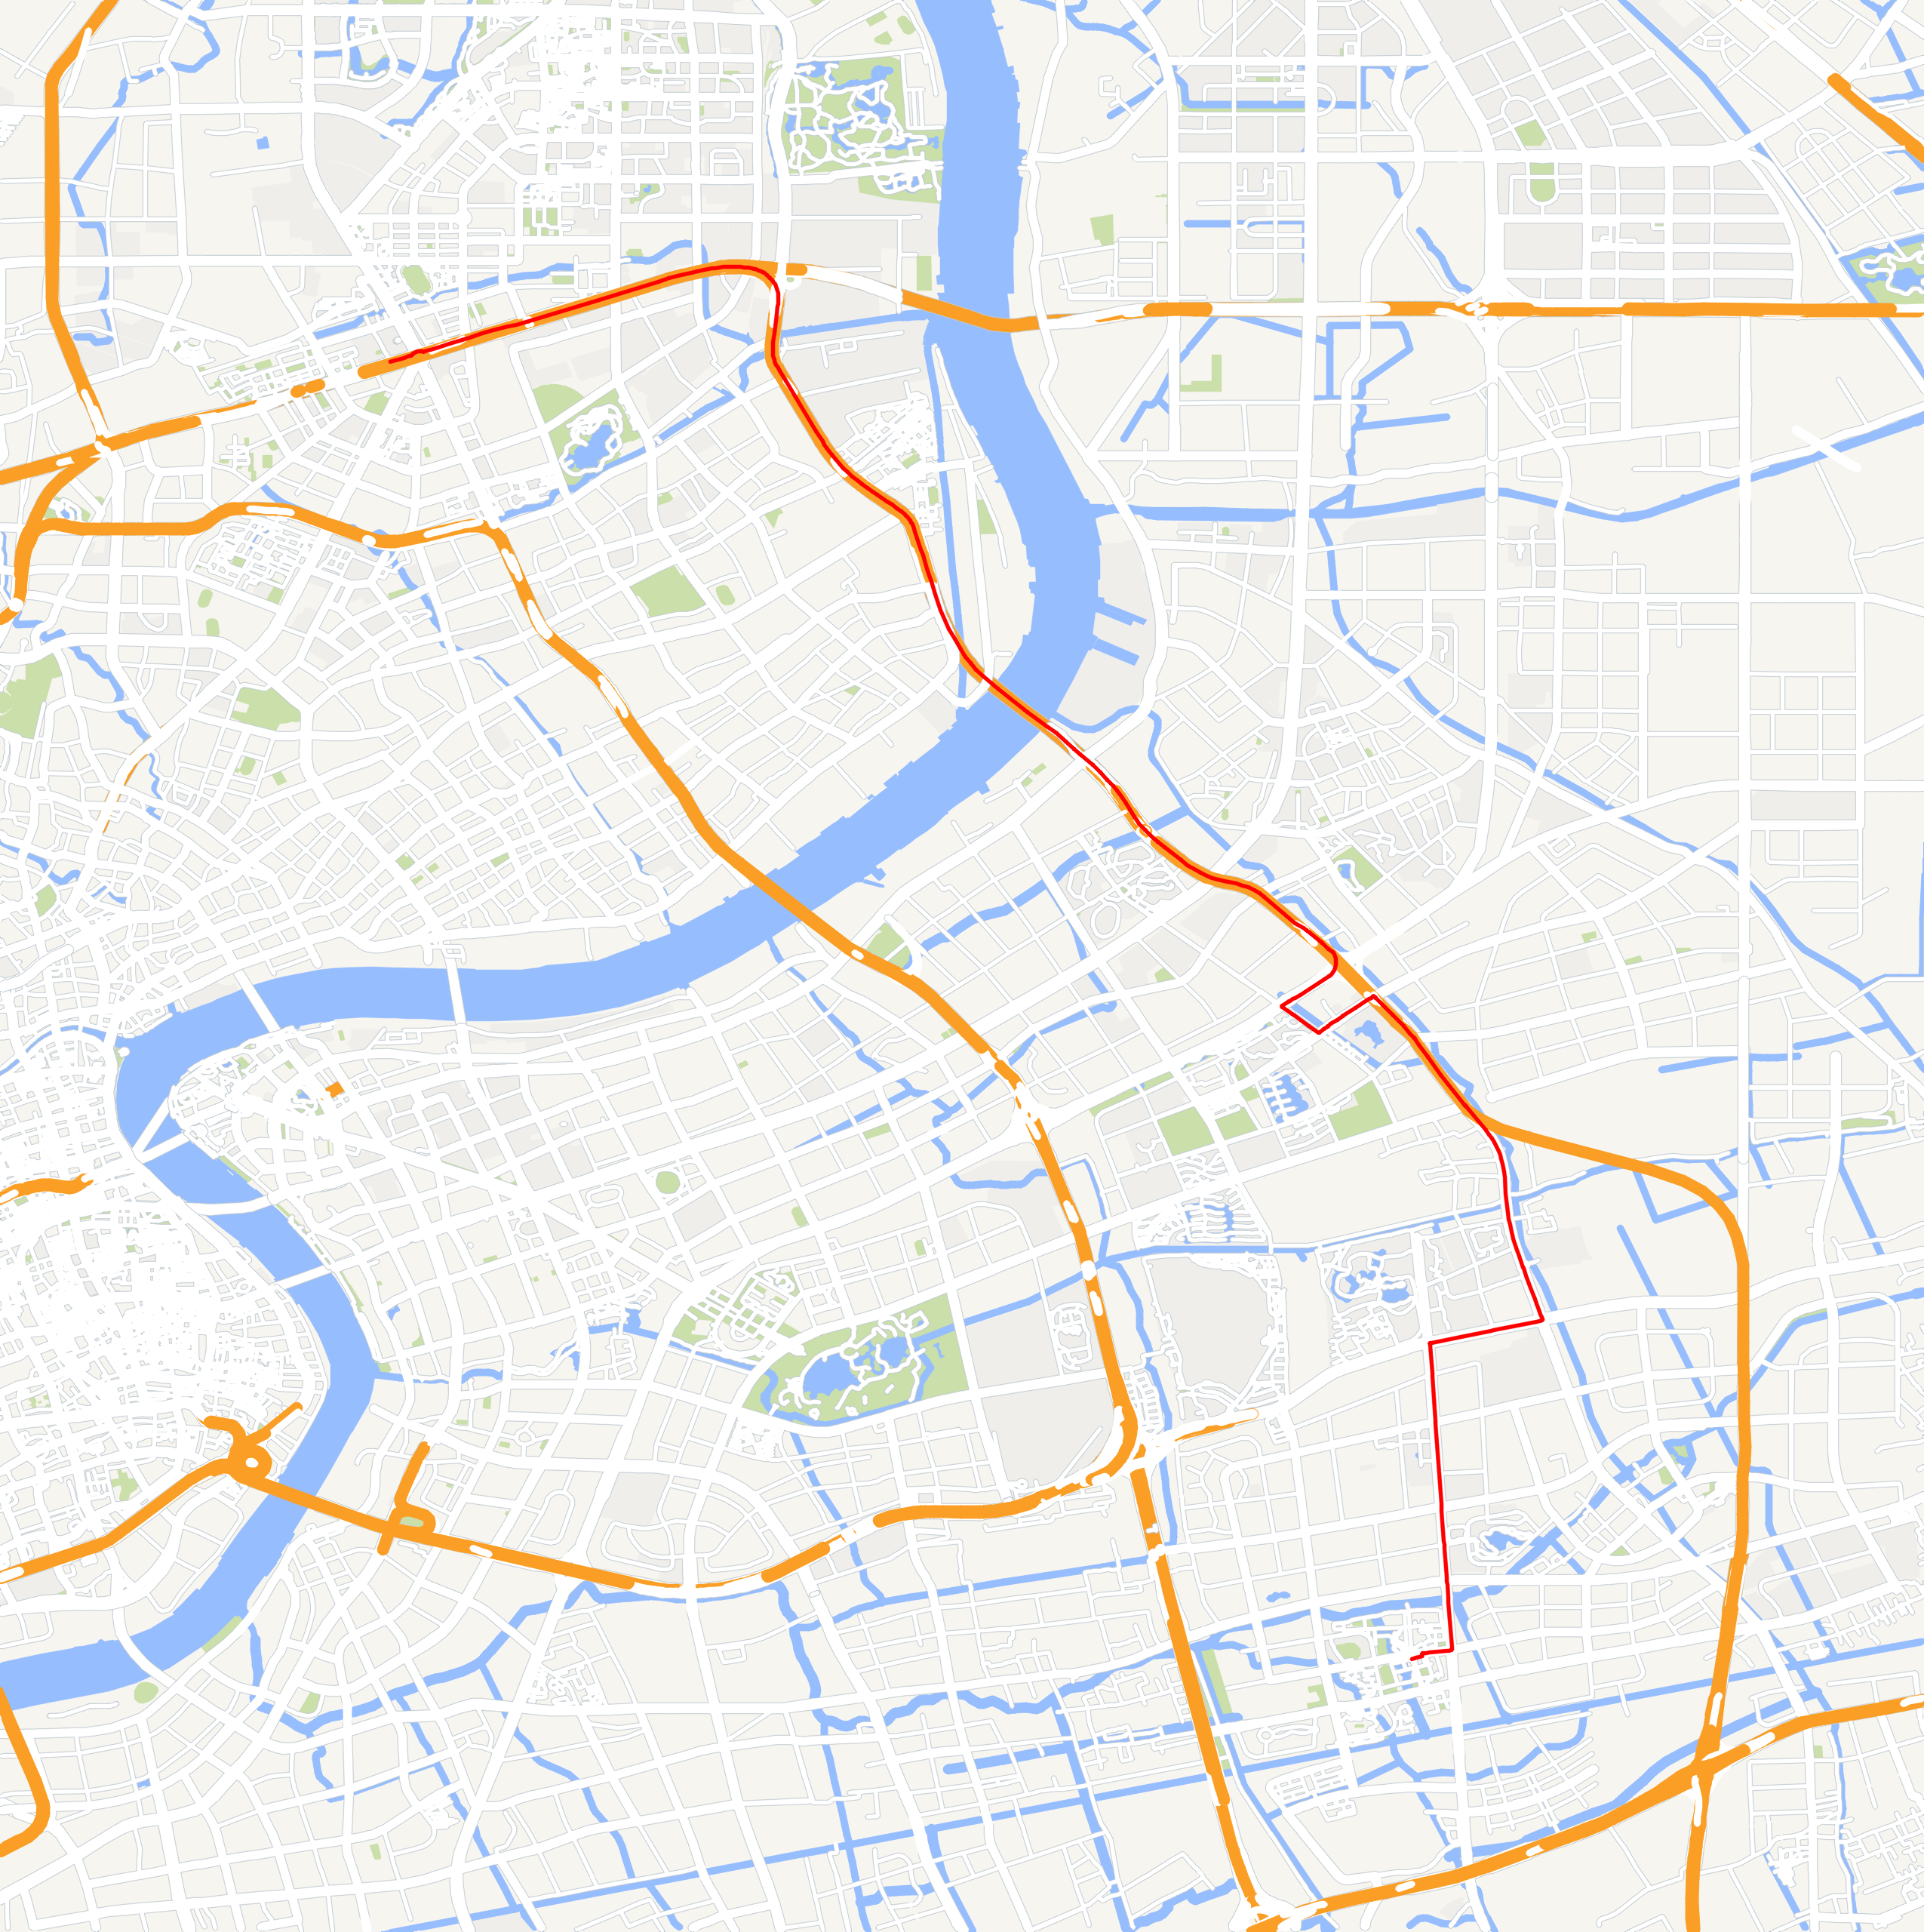
\includegraphics[width=0.4\textwidth]{张江到邯郸绕}}
\subfigure[相关信息]{
\label{Fig.sub.8}
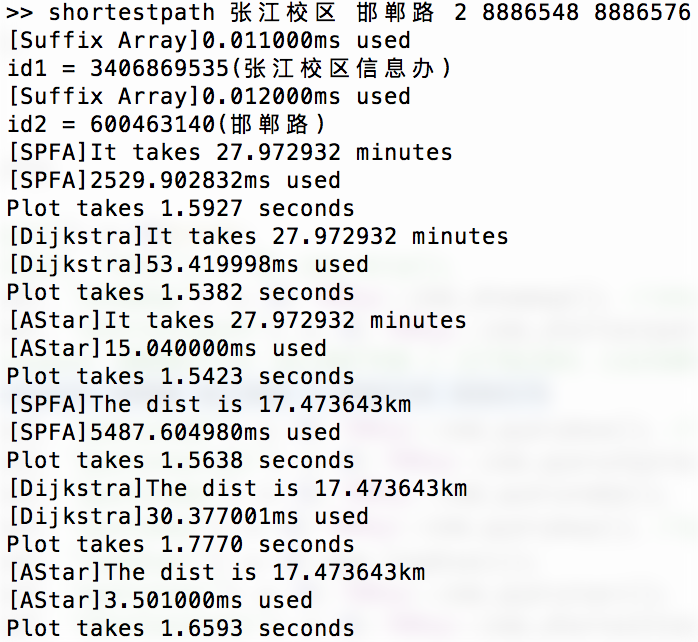
\includegraphics[width=0.4\textwidth]{张江到邯郸绕路}}
\caption{张江到邯郸最短路(躲避拥堵的杨浦大桥)}
\label{Fig.lable4}
\end{figure}


\section{出租车轨迹数据管理}
\subsection{做法概要}
根据出租车轨迹文件的特点,直接用数组存储,二分查询即可\footnote{当然使用1707个vector存储就不用二分,直接按地址查找就好了,但是这样也会涉及ID和下标之间的映射问题,并不一定会快很多}。经统计可知一共有1707辆出租车的13294680条左右的采样点信息。所以如果只是查询一条轨迹并且把它显示出来的话并不需要特殊的数据结构,只要二分出某一出租车数据开始的位置,然后取出需要的兴趣点即可。实测这样查询一条完整的出租车24小时的路径只需要0.7ms的时间。最终实现的功能是可以查询某一出租车在一段时间之内的轨迹数据并且显示在图上,还可以查询第i个数据点的相关信息。显示效果如图。

\begin{figure}[htbp] 
\centering\includegraphics[width=2.9in]{taxipath} 
\caption{10944号出租车下午1点到晚上11点的行驶轨迹}\label{fig:2} 
\end{figure} 


虽然本题可以这么简单的实现,但是这和实际情况并不完全符合,因为分析数据时并不会只查询一条出租车的路径,而会像之前我处理地图数据时一样查询给定二维空间内的数据点,甚至是三维空间(加上时间这一维,在最后一题中会有涉及)内的数据点。再加上后面的任务中也涉及到范围查询的问题,所以我认为仅仅调用R树的库是不足以说明问题的,所以我写了几种数据结构来对比它们的性能,详细分析见范围查询一节。

\section{范围查询}
\subsection{实验方法概述}
因为地图中只有50000个点,为了在不同规模的数据集上进行测试,我选择了给出的出租车数据文件。出租车数据文件大小为1G,有大约13293000个点,可以通过截取数据的不同部分来获得不同规模的数据。编译时开O2优化。
\subsection{R树}
调用了Boost库中的R树,R树的结点分裂算法有线性、二次方和R*三种,叶节点个数M也是可以修改的。下面用500万个点随机询问10000次的时间来代表查询性能。

\begin{tabular}{|l|l|l|l|}
\hline
结点分裂算法 & linear & quadratic & rstar \\
\hline
建树时间    &  6s    &  7s       & 17s    \\
\hline
查询时间    &  28s   &  26s      & 44s    \\
\hline
\end{tabular}

上面实验是在叶节点个数为16时得到的,通过对叶节点个数的实验发现,叶节点个数大于20时查询时间都差不多逐渐趋近于24s,但是建树时间越来越长。最后选择了20个子节点的quadratic。

\subsection{线段树套红黑树}
按照坐标点的横坐标为关键字建立一棵线段树,在每个线段树区间的节点上挂一棵以纵坐标为关键字的红黑树(红黑树中的元素满足横坐标在线段树区间内)。查询时通过线段树可以找到满足在横坐标范围内的点,再通过红黑树找到纵坐标在查询范围内的点。

这样的话空间复杂度为$O(nlog_2n)$,因为每个节点都最多出现在$log_2n$个区间中,所以最多出现在$log_2n$棵红黑树中。

查询的时间复杂度为$O(log_2n*log_2n)$,因为最多进入$log_2n$个结点在红黑树中查找需要$O(log_2m) <= O(log_2n)$(m为红黑树结点个数)所以上面提到的复杂度其实是一个上界,实际复杂度可能会比这个小。

\subsection{线段树套有序数组}
将其实现后稍加思考可以发现,上面做法中的红黑树的用处只是找到纵坐标满足条件的点,所以如果用有序数组替换红黑树只要用二分查找的方法就可以达到同样的功能,虽然复杂度不变,但是常数应该会比红黑树小很多。

\subsection{fractional cascading}
fractional cascading\cite{ wiki:xxx}是一种基于上述数据结构的优化技巧,通过一定的预处理,可以把时间复杂度优化到$O(log_2n)$。而且这种优化可以很容易的扩展到多维的情况,即k维的复杂度为$O(log_2n^{k-1})$。

主要想法是发现其实在线段树结点内的每次二分查找并不是必要的,因为每次二分查找所要找的纵坐标是一样的,所以可以通过线段树结点的父结点查找出的边界直接O(1)的给出子结点的边界。

具体详细做法参见附录。

\subsection{效率对比}
\begin{tabular}{|l|l|l|l|l|}
\hline
序号 & 算法 & 点数 & 询问数 & 询问时间 \\
\hline
1   & 线段树套红黑树 & 13293000 & 1000 & 63s \\
\hline
2   & 线段树套有序数组暴力 & 13293000 & 1000 & 25s \\
\hline
3   & 线段树套有序数组二分 & 13293000 & 1000 & 16s \\
\hline
4   & fractional cascading & 13293000 & 1000 & 15s \\
\hline
5   & R树 & 13293000 & 1000 & 53s \\
\hline
\end{tabular}

\begin{tabular}{|l|l|l|l|l|}
\hline
序号 & 算法 & 点数 & 询问数 & 询问时间 \\
\hline
1   & 线段树套红黑树 & 5000000 & 1000 & 19.7s \\
\hline
2   & 线段树套有序数组暴力 & 5000000 & 1000 & 6.9s \\
\hline
3   & 线段树套有序数组二分 & 5000000 & 1000 & 5.3s \\
\hline
4   & fractional cascading & 5000000 & 1000 & 4.9s \\
\hline
5   & R树 & 5000000 & 1000 & 18.5s \\
\hline
\end{tabular}

实验的结果和我想象的基本相同,但是fractional cascading的效果不如我想象的好。

我觉得可能的原因有这么几点:一是程序3的空间复杂度虽然并不增加,但是常数大概是别的程序的3倍,因为点数很多所以会更多的使用虚拟内存(本机内存共8GB,当点数为5000000时已经占用了5GB的内存,当点数为13293000时占用了12GB内存),因为磁盘的读取速率比内存慢很多,所以程序运行速度会因此而变慢,可以推测出如果在内存够用的情况下程序4是会优于程序3很多的,但是如果使用较小数据来测试发现两者(程序3,4)所花的时间几乎是一样的,没有太多的差异;二是程序的测试数据是随机生成的,所以数据中询问的范围会比较大,这样会在时间复杂度中添加O(查询所得点数项),使得最后得到的询问时间加了这一项后显得不正常。

通过以上分析,基本可以认为fractional cascading的效果虽然没有想象的好(像分析的一样去掉一个log的效果),但是也比实验上看上去的要好。

通过这个实验我明白了:程序的运行时间确实受到很多条件的影响,虽然最后结果和预想的不完全一样,但是还是可以根据上面的分析说明加了ractional cascading优化之后确实效果要比单独的二分查找要好一些。

总之,程序4最快,大概是R树的几倍,而且随着点数的增多优势在不断增大。红黑树的常树数太大导致实际效果比R树还差。

\subsection{范围查询在地图中的应用}
如果地图上的兴趣点是动态增加的,而且增加的频率很快,且要求实时更新,那么应该选用R树这样的可以动态增删结点的数据结构。而如果是静态的或者是不要求实时性的就可以选用上面提到的比较好写也比较快的数据结构。

在实际实现上还是选择了R树,是因为在分析各种范围查询复杂度之前已经使用了R树,就不想再换了。而且对于这个数据规模,各种数据结构之间的差异其实不是很明显,使用R树还可以支持随时插入兴趣点。但是如果有海量兴趣点的话就要考虑数据结构的选择问题了。因为地图数据中真正的兴趣点不是很多,所以把所有路上的结点作为兴趣点来使用。范围查询效果图如图5所示。

因为选择了R树,所以同时实现了插入新兴趣点的功能。

\begin{figure}[htbp] 
\centering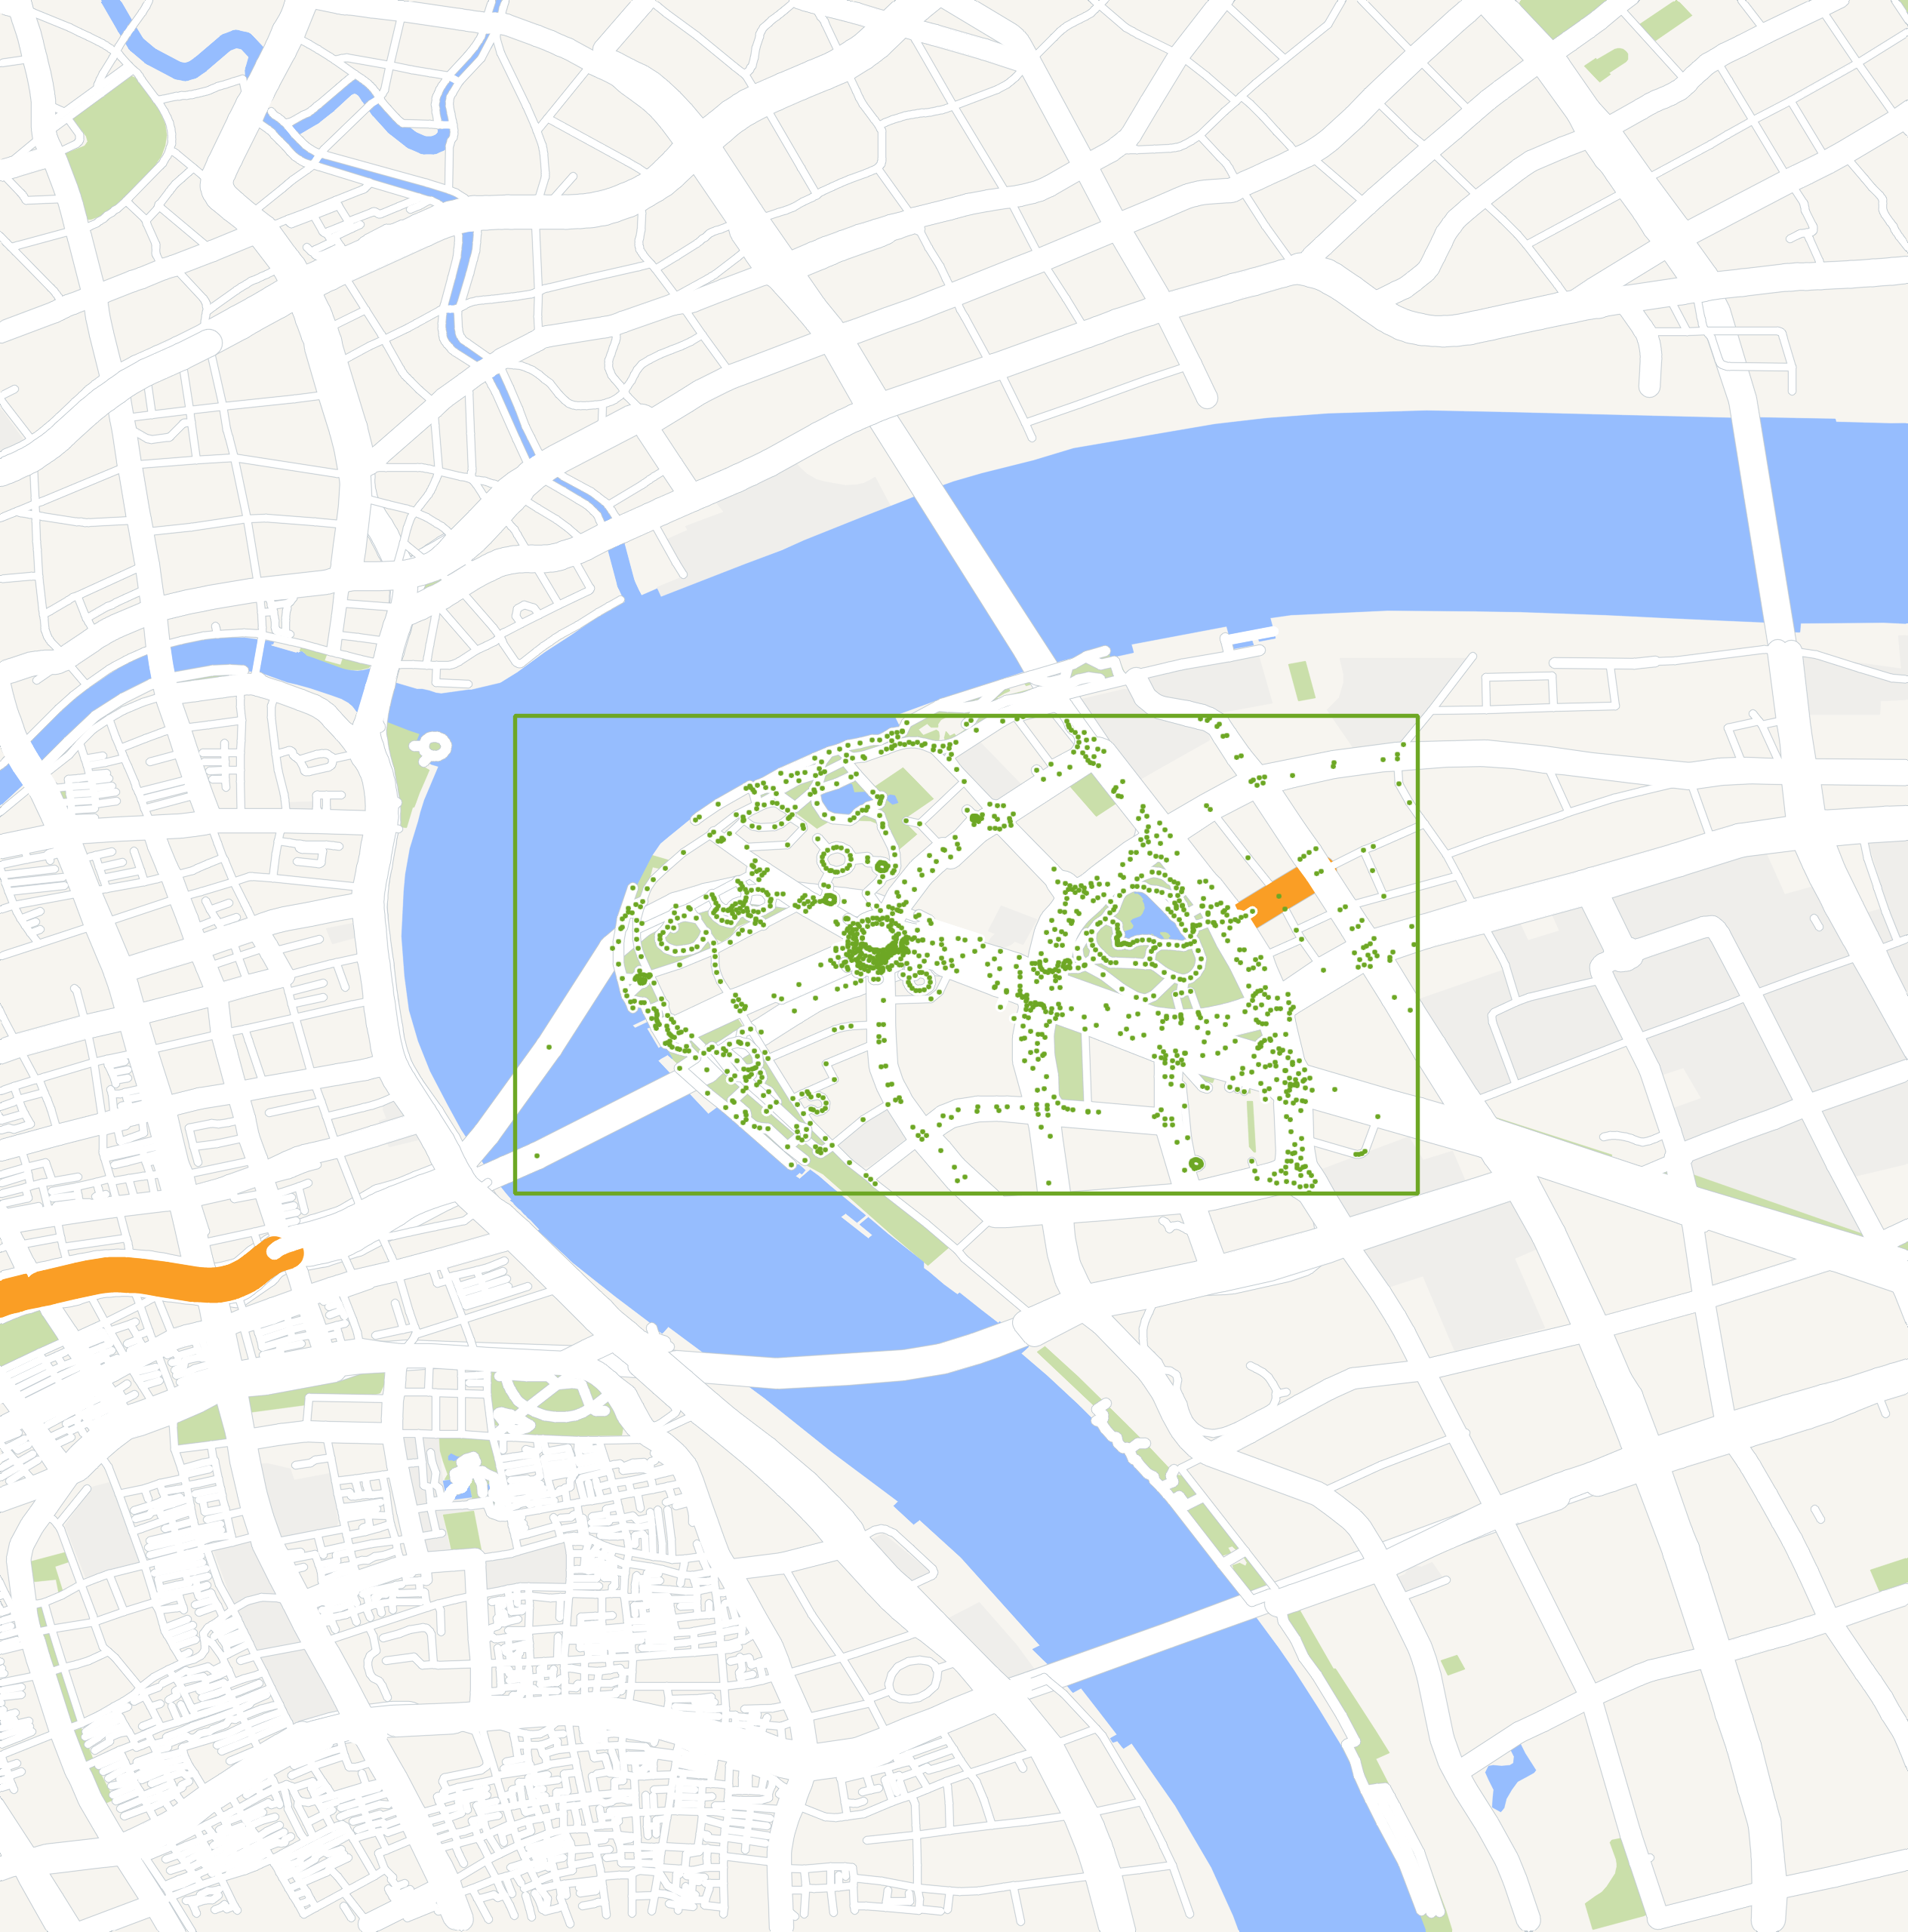
\includegraphics[width=2.9in]{querybox} 
\caption{范围查询效果图}\label{fig:3} 
\end{figure} 

\section{近邻查询}
近邻查询使用的也是R树实现的,支持K近邻查询,查询所需时间和k有关,具体关系如下:\\
\begin{tabular}{|l|r|r|r|r|r|r|r|}
\hline
k & 1 & 10 & 100 & 1000 & 10000 & 100000 & 1000000 \\
\hline
time(ms) & 0.026 & 0.036 & 0.1 & 0.578 & 5.80 & 20.25 & 16.13 \\
\hline
\end{tabular}

在地图上显示效果如图所示。红圈为查询的中心点,绿色的点为周围的1000个近邻点。
\begin{figure}[htbp] 
\centering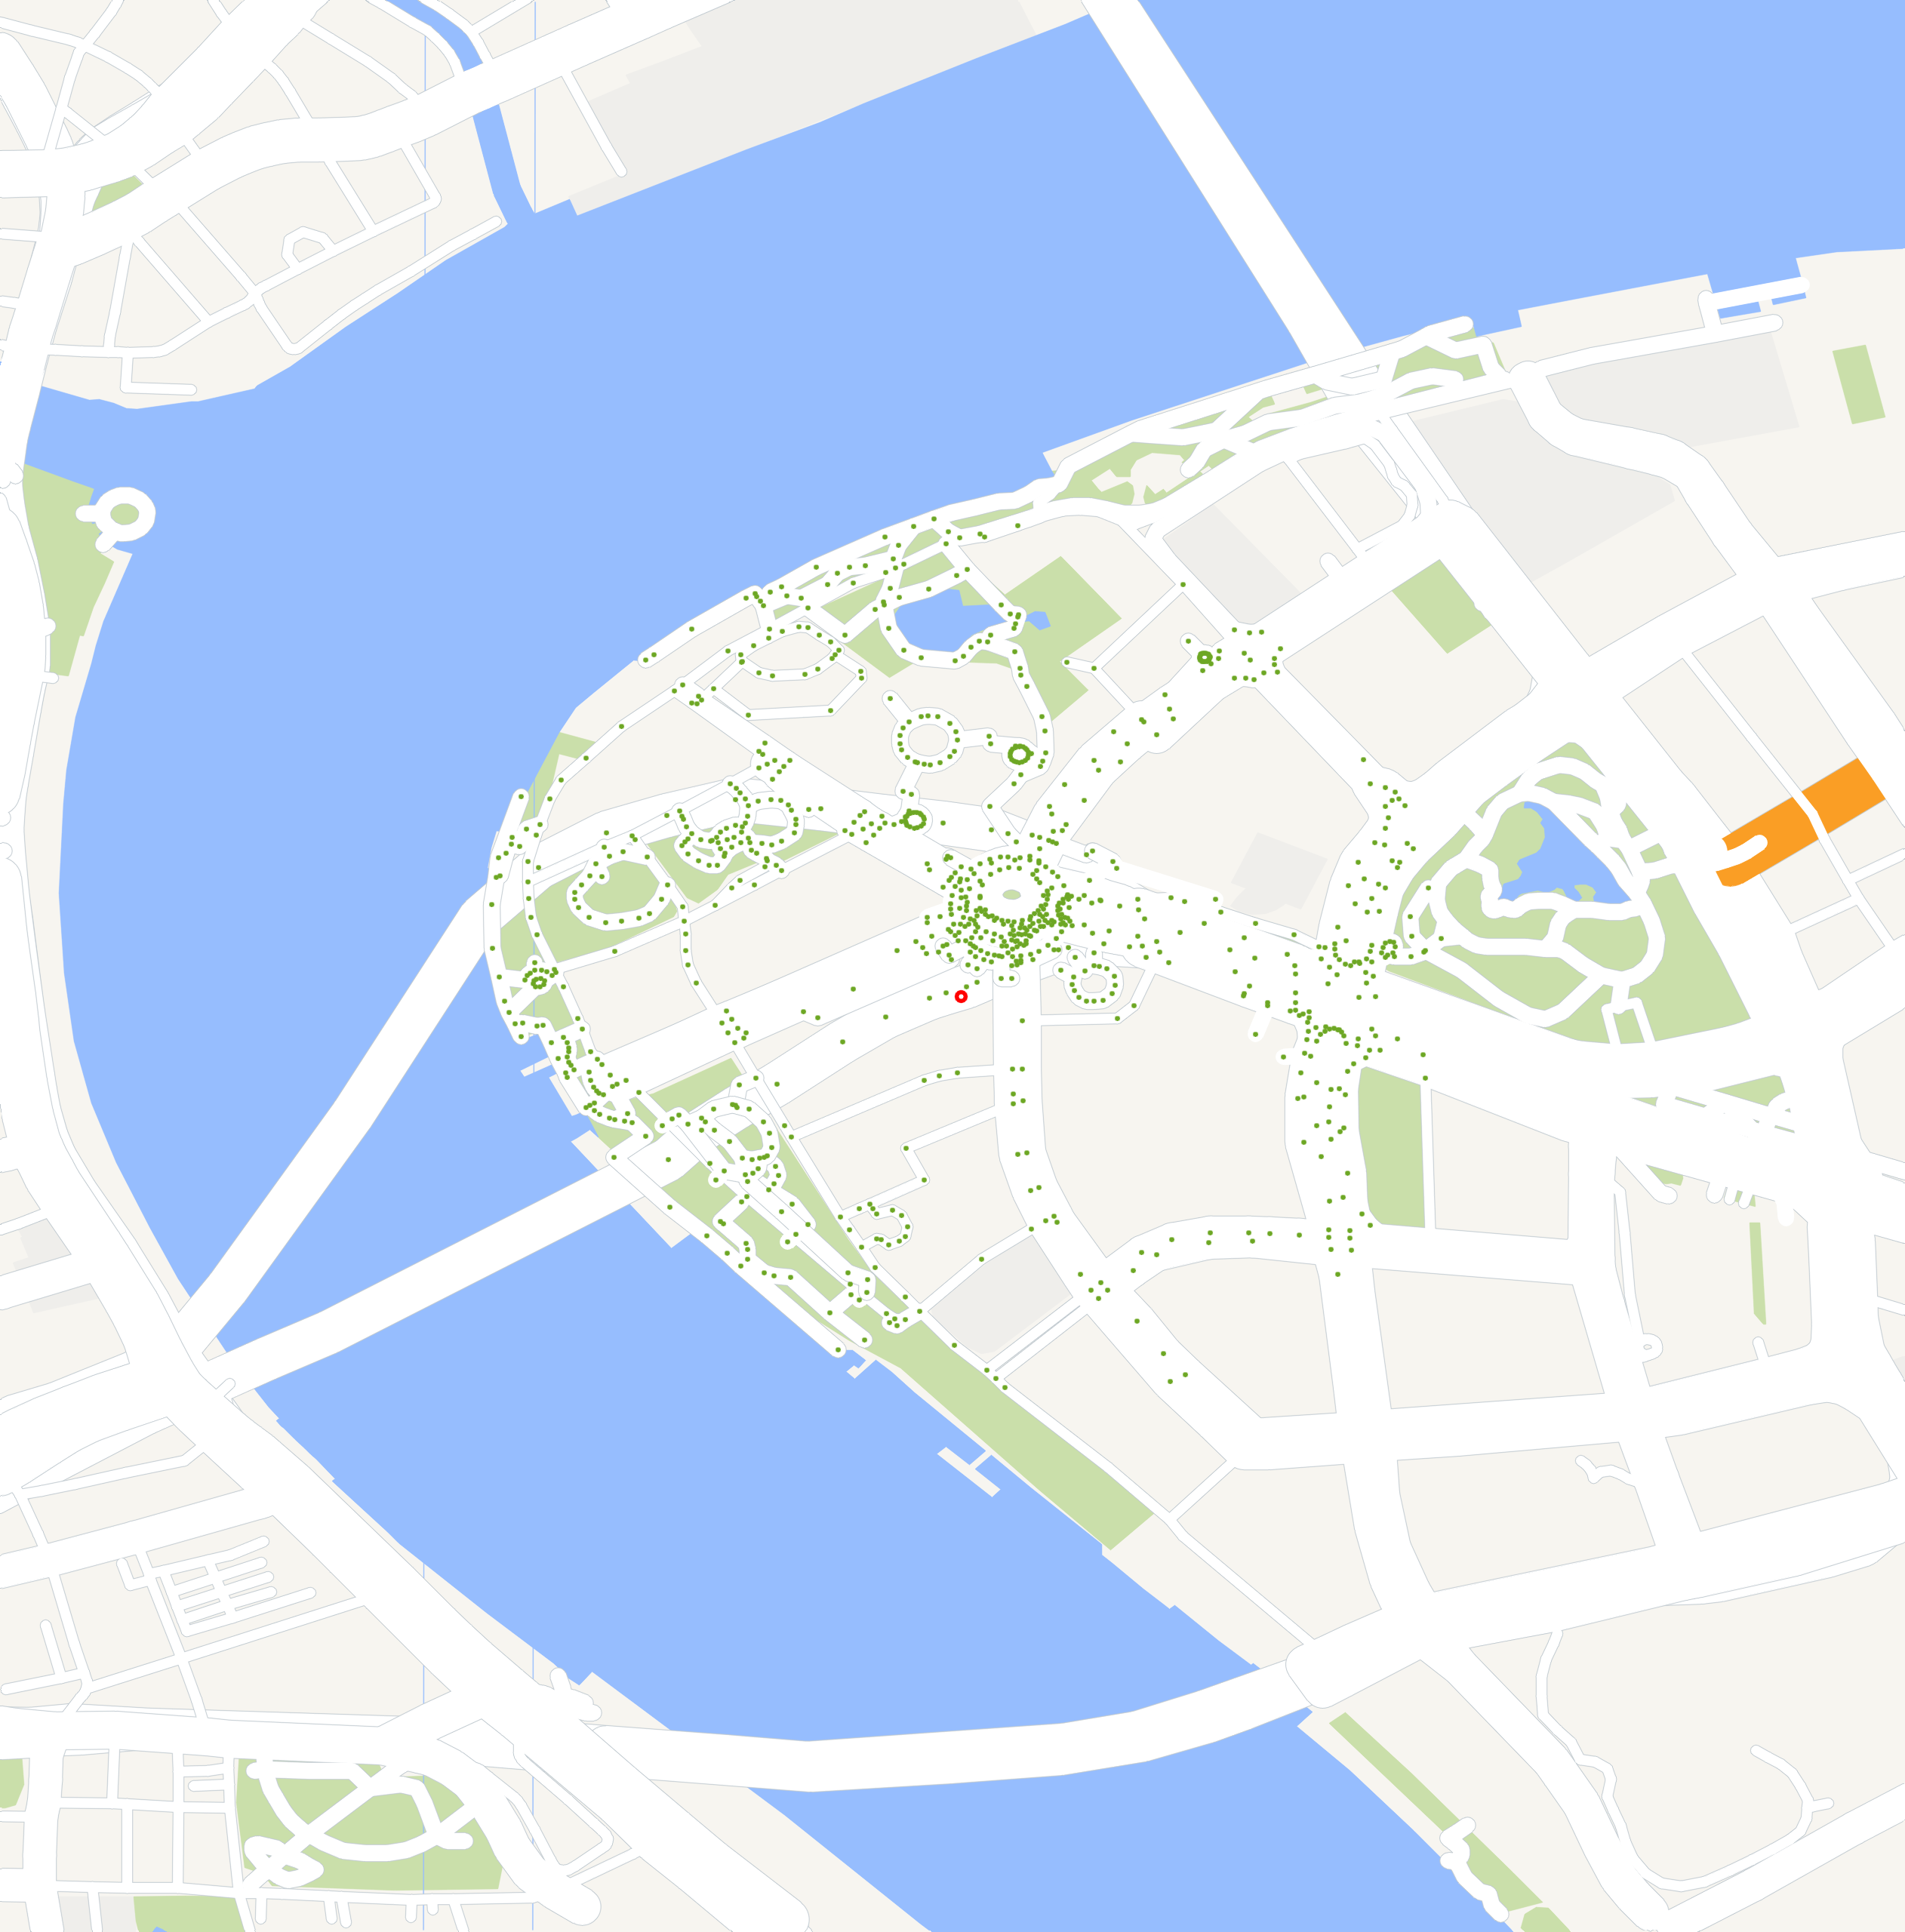
\includegraphics[width=2.9in]{nearest} 
\caption{k-邻近查询效果图}\label{fig:4} 
\end{figure} 
\section{挖掘和分析——哪里更能拉到客?}
\subsection{功能描述}
针对出租车司机经常有载不到客的情况,我设计的一套系统可以基于出租车的轨迹数据为在某一特定时间特定地点的空车司机推荐附近更容易拉到客人的点。具体来说就是给出当前点和当前时间就可以给出附近更容易接到客人的点,并且显示在地图上。

\subsection{实现方法——三维kd树}
完成这一任务主要使用的数据结构是三维kd树,三维是时间的一维和空间的两维。首先把所有载客点加入kd树中,载客点的判断标准是这个时刻的点不是空车,而上个时刻是空车。当获取到一次询问时查询在这个时间点周围一段时间内的载客点。然后对每个载客点算出在它周围邻域内载客点的密度,最后选密度大的一些点作为推荐。更具体一点是如果周围点数高于平均,那么用周围点个数减去平均值的二倍再除以最大值乘以六;否则取负无穷。然后放到sigmoid函数里面,目的只是使大于某一阈值的点尽可能红,其它点有从红到白的渐变而已。

\subsection{效果展示}
图为在中午13点在复旦大学的询问请求,点的桃红色颜色越深就代表自信度越高。通过看图可以发现周围三个主要的接客点分别是五角场万达广场门口、控江路江浦路的上海新华医院以及长海路黑山路上的长海医院,而其他时段就不一样了。中午在五角场和医院打车的人多都非常好理解。

\begin{figure}[htbp] 
\centering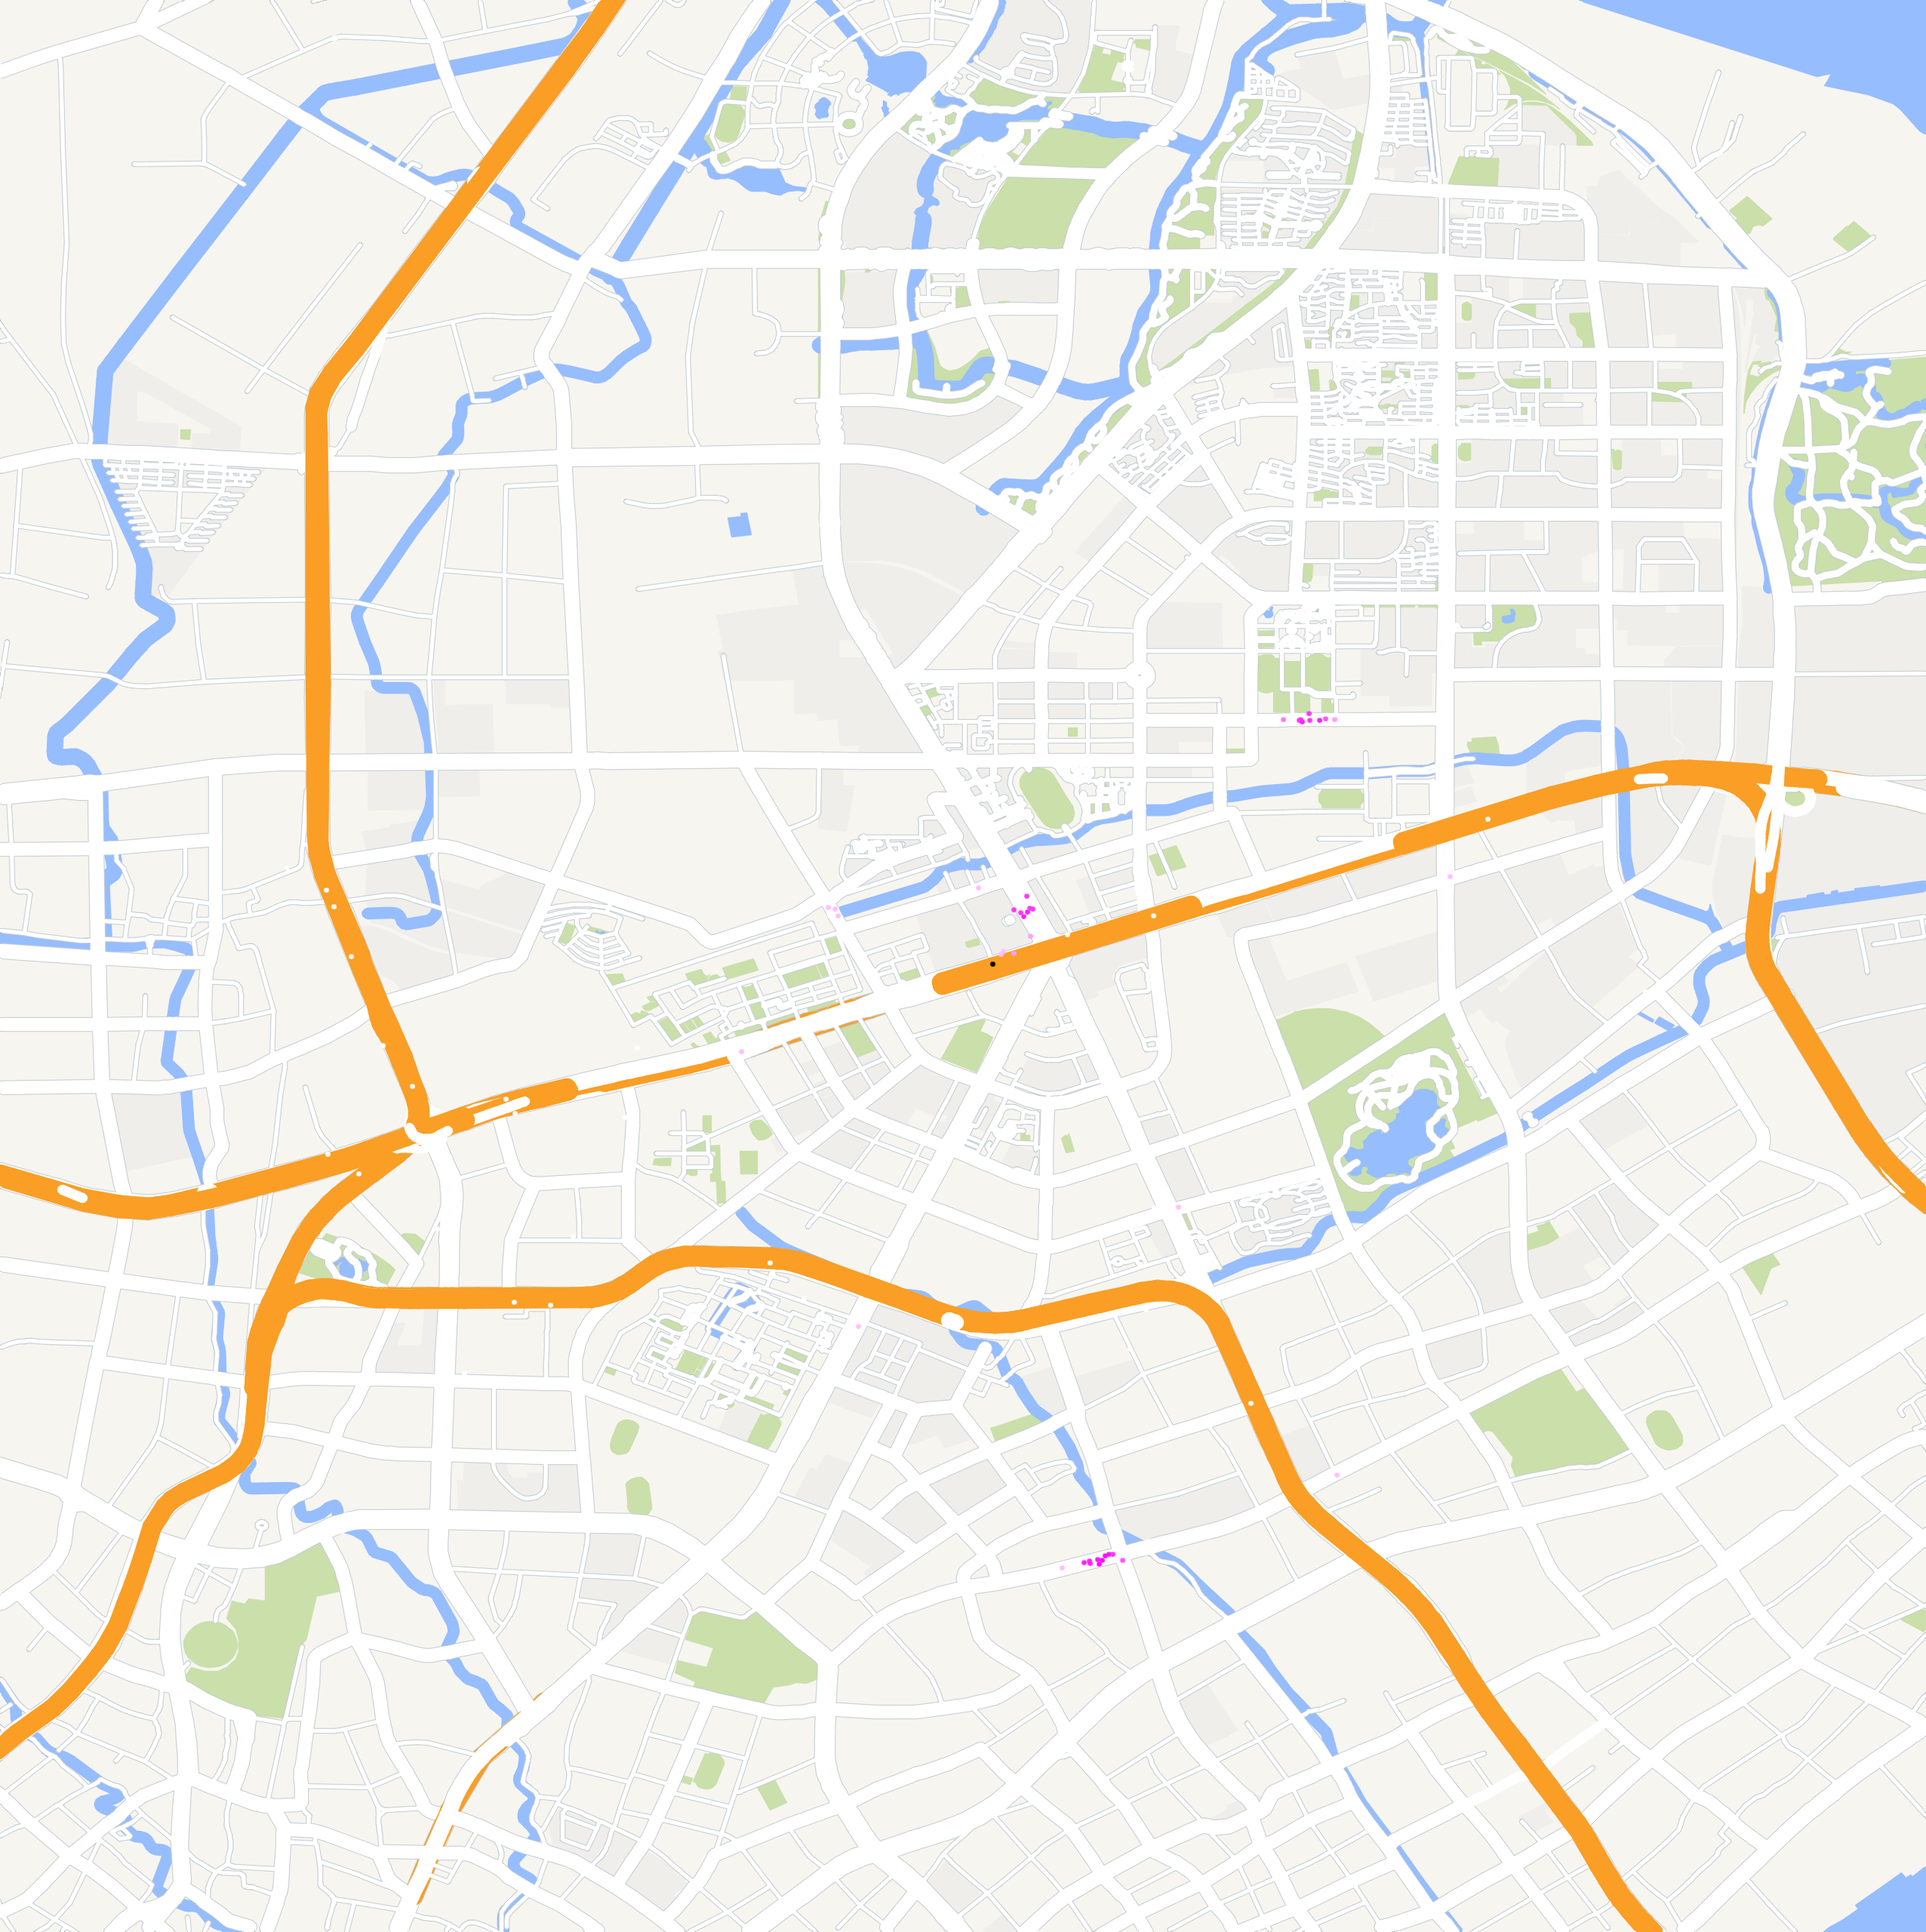
\includegraphics[width=2.9in]{taxirecommend} 
\caption{拉客位置推荐-中午一点复旦大学周边}\label{fig:5}
\end{figure} 

\section{其它}
通过后缀数组实现了兴趣点名字的查询,比如输入“小学”就会查到所有名字中带有“小学”的兴趣点坐标。

做的是命令行ui,操作起来相对麻烦一些。

\section{[附录一]实验环境以及相关配置说明}
\begin{figure}[htbp] 
\centering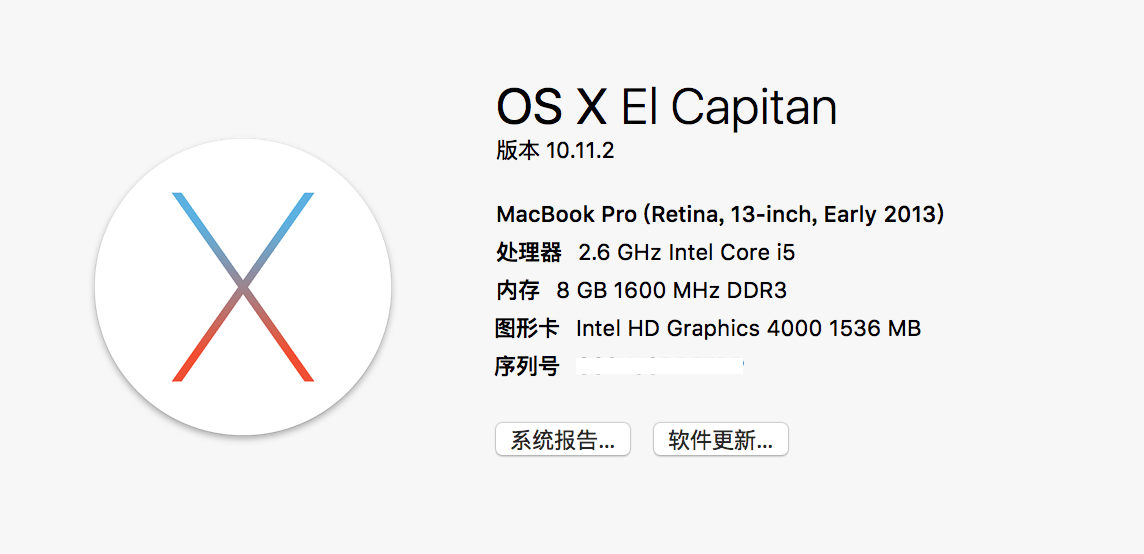
\includegraphics[width=2in]{实验电脑配置} 
\caption{笔记本电脑相关}\label{fig:6}
\end{figure} 
\begin{figure}[htbp] 
\centering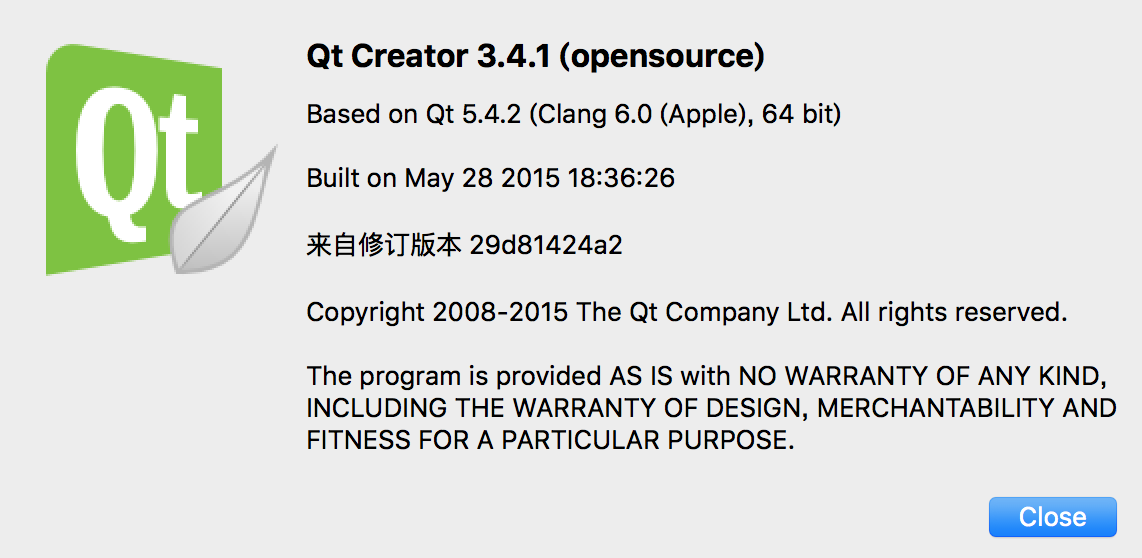
\includegraphics[width=2in]{IDE环境} 
\caption{IDE环境}\label{fig:7}
\end{figure} 
\begin{figure}[htbp] 
\centering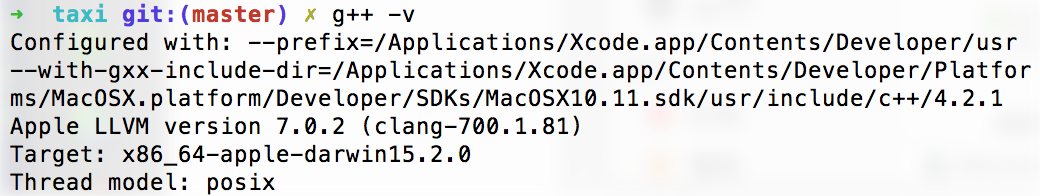
\includegraphics[width=2in]{编译器} 
\caption{编译器}\label{fig:8}
\end{figure} 

相关环境如图所示,之后需要安装opencv2和boost库,最后直接把LiMap、NearestNode.conf、plot\_config.xml、shanghai\_map.xml、shanghai\_taxi\_20150401.csv放到一个文件夹下,最后从命令行中打开这个文件夹最后输入命令./LiMap即可运行。

\section{[附录二]软件使用说明}
打开软件后输入help查看,内容如下:
\begin{lstlisting}
显示地图:
    语法:showmap lat lon level
    解释:level是缩放级别,取值为11到18
    举例:
        showmap 31.30186 121.51159 13

查最短路:
    语法1:shortestpath id1 id2 n ...
    解释1:id1 id2为两个node的id,n为拥堵路的数量,后面跟n个数代表拥堵路的id
    举例1:shortestpath 1008057714 1813887498 2 227962891 11635095
    语法2:shortestpath s1 s2 n ...
    解释2:s1 s2是点的名称,其它同上
    举例2:shortestpath 邯郸路 张江校区 2 8886548 8886576

通过名字找坐标和id:
    语法:queryname name
    举例:queryname 复旦

查询道路:
    语法:queryway name/id
    举例:queryway 肇嘉浜路
        queryway 世纪大道
        queryway 272231909

范围兴趣点查询:
    语法:querynode maxlat minlon minlat maxlon
    举例:querynode 31.2449 121.4886 31.2349 121.5073

k邻近兴趣点查询:
    语法:querynearest lat lon k
    举例:querynearest 31.2392 121.4956 100

最短路性能测试:
    语法:shortesttest n
    说明:随机生成起点和终点,测试n次不同最短路算法
    举例:shortesttest 20

插入兴趣点:
    语法:insertpoint lat lon
    举例:
        querynode 31.2449 121.4886 31.24 121.49
        insertpoint 31.2440 121.489
        querynode 31.2449 121.4886 31.24 121.49

以下为出租车相关,在使用以下功能前先输入loadtaxi载入出租车轨迹信息

查询一辆出租车轨迹:
    语法:querytaxi taxiid starttime endtime n ...
    说明:n为要查询的点的个数,后面n个数字,代表查询第几个点
    举例:querytaxi 10944 0:0:1 23:59:59 2 2 3(最后三个数字代表,输出两个点的信息,分别是第二个点和第三个点)

查询去哪里载客:
    语法:queryneartaxi lat lon r time duration
    说明:r是搜索半径 time是当前时间 duration是设置搜索范围的时间长度
    举例:queryneartaxi 31.2363 121.4690 0.01 21:0:0 3600
    上例为当前时间为21点,所以搜索范围为20点半到21点半

输出得图片可以在同一文件夹中找到对应或相似的文件名
\end{lstlisting}

\section{[附录三]文件总览}
如图13、图14。
\begin{figure}[htbp] 
\centering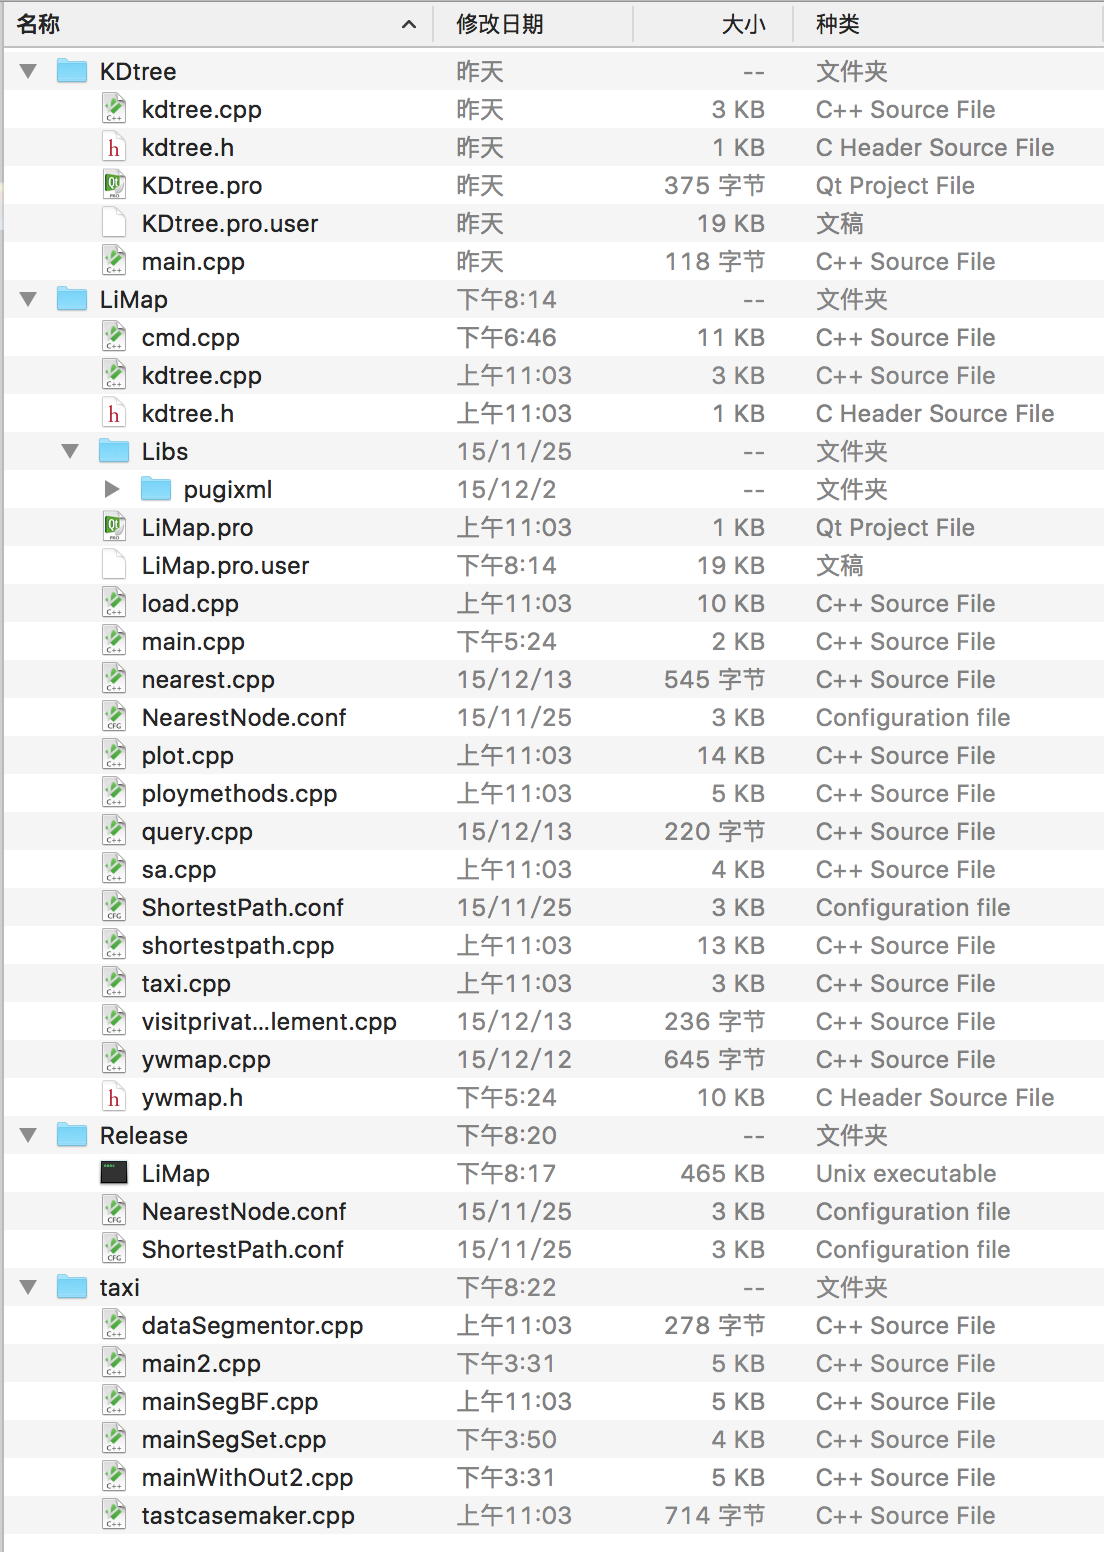
\includegraphics[width=4in]{文件一览} 
\caption{文件总览}\label{fig:9}
\end{figure} 

\begin{figure}[htbp] 
\centering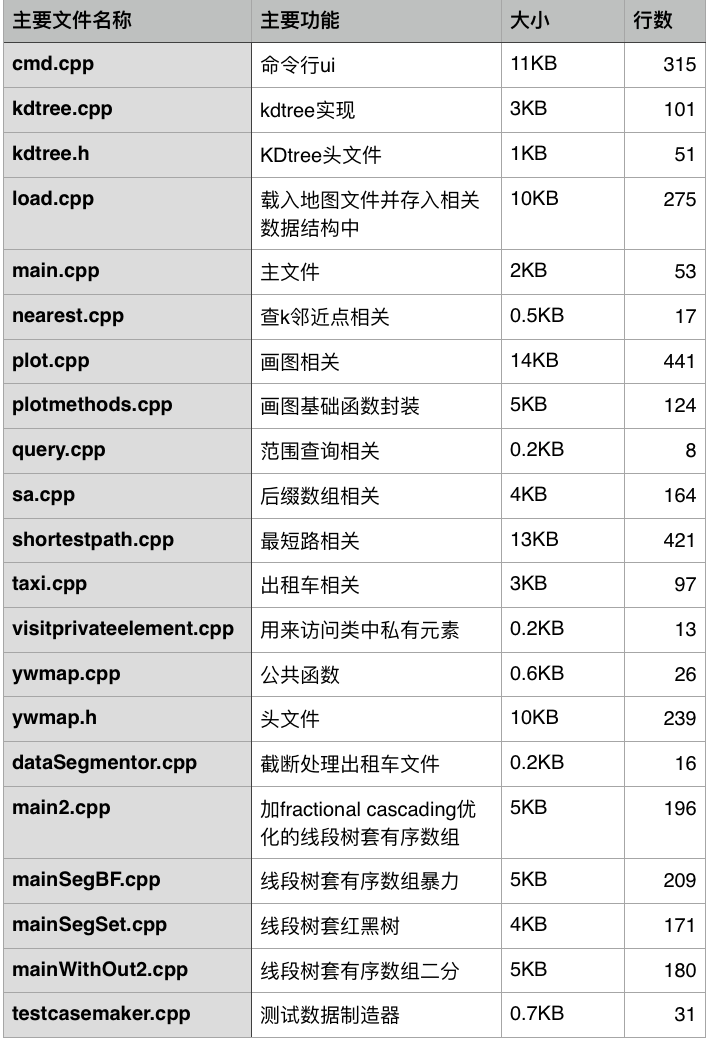
\includegraphics[width=4in]{表格文件总览} 
\caption{主要文件功能}\label{fig:10}
\end{figure} 

\section{[附录四]fractional cascading优化}
先考虑这么一个问题,假设有两个数组$A_1$和$A_2$且$A \subseteq B$,我们要在A和B中查找大于等于x的元素有多少。朴素的方法是二分两次。但是其实通过预处理给A中每一个元素一个指向B中元素的指针满足如果$a_i -> b_j$那么$a_i \leq b_j$且$a_i > b_{j-1}$即a指向b中大于或等于a的第一个元素。

对于线段树的每个节点v,套一个单调数组p,记录的是y坐标,对于p中每个元素附带两个指针ptl和ptr,分别指向其左儿子中不比p[i]小的第一个元素和其右儿子中不比p[i]小的第一个元素。

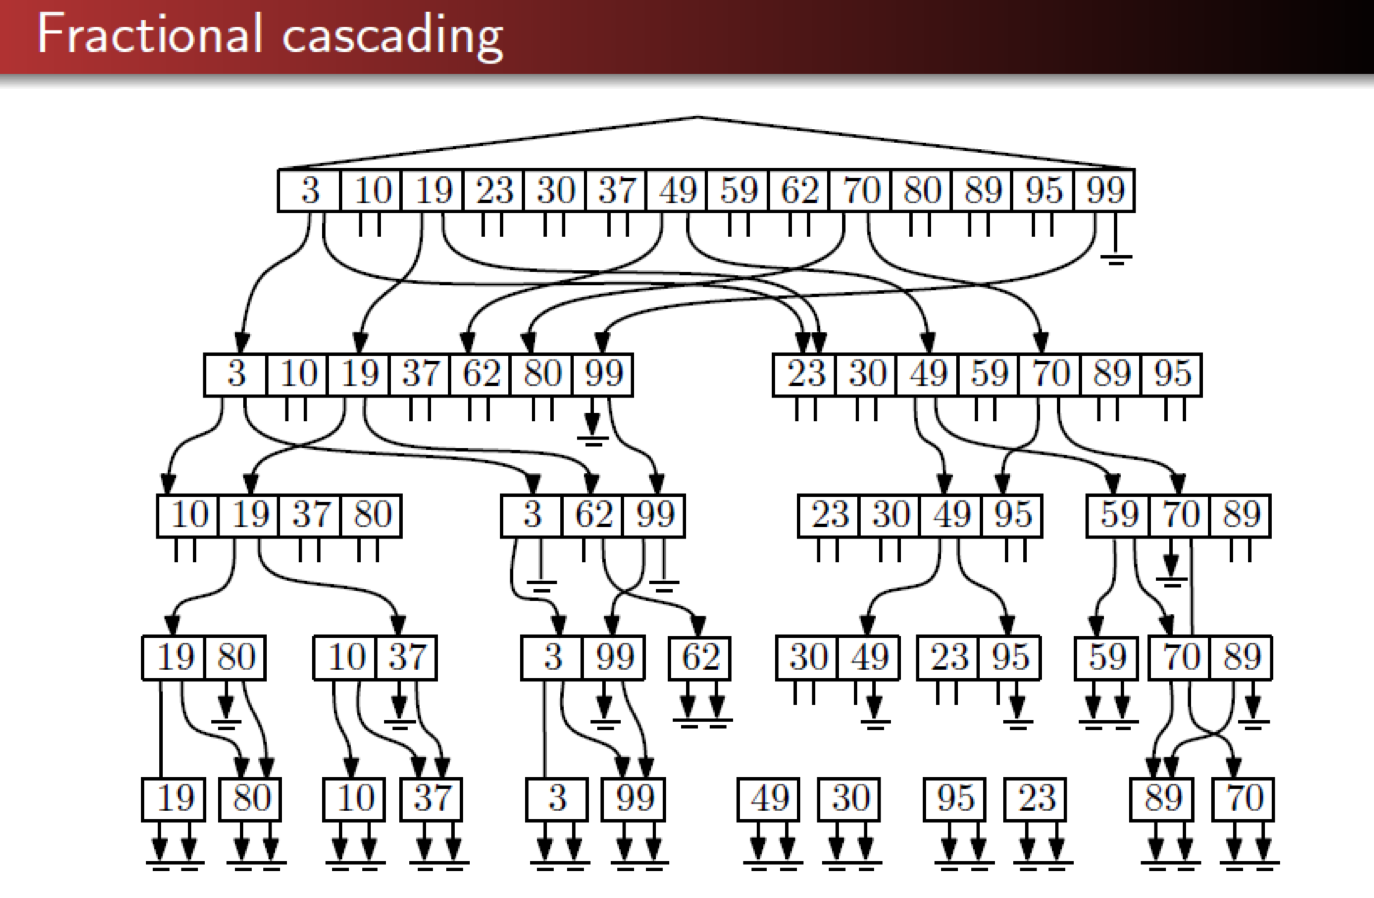
\includegraphics[width=4in]{fractional} 

这样,在查询时就不用每次都去二分了,而可以通过父节点的指针直接定位到第一个有效元素。这样只需要在根节点处二分就可以一劳永逸了。总的查询复杂度为$O(log_2n)$。

\bibliography{mybibtex}
\end{document}

